% Alder -- a fourth-round proof-language proposal.
% Build: latexmk -pdf -interaction=nonstopmode -halt-on-error Alder.tex
% Self-contained article; bibliography embedded; no external figures required.
\documentclass[11pt,a4paper]{article}
\usepackage[T1]{fontenc}
\usepackage[utf8]{inputenc}
\usepackage{lmodern,microtype}
\usepackage[margin=24mm,headheight=15pt]{geometry}
\usepackage{amsmath,amssymb,amsthm,mathtools,stmaryrd}
\usepackage{booktabs,tabularx,longtable,array}
\usepackage{xcolor,listings,fancyhdr,titlesec,enumitem,needspace,etoolbox}
\usepackage{tikz}
\usetikzlibrary{arrows.meta,positioning}
\usepackage{xurl}
\usepackage[colorlinks=true,linkcolor=oliveink,citecolor=oliveink,urlcolor=oliveink]{hyperref}
\usepackage{bookmark}
\definecolor{oliveink}{HTML}{465340}
\definecolor{ink}{HTML}{26312C}
\definecolor{muted}{HTML}{626B62}
\definecolor{paperpanel}{HTML}{F4F3ED}
\definecolor{rulegray}{HTML}{CCD0C5}
\hypersetup{pdftitle={Alder: Residual Types and Proof-Producing Mathematical Elaboration},pdfauthor={GPT-6 Astra Pro, for Vladimir Reshetnikov},pdfsubject={Fourth-round proof-language proposal; refinement types, residual inference, certified computation and synthesis},bookmarksnumbered=true}
\titleformat{\section}{\Large\bfseries\sffamily\color{oliveink}}{\thesection}{.65em}{}
\titleformat{\subsection}{\large\bfseries\sffamily\color{ink}}{\thesubsection}{.65em}{}
\titleformat{\subsubsection}{\normalsize\bfseries\sffamily\color{ink}}{\thesubsubsection}{.65em}{}
\titlespacing*{\section}{0pt}{2.8ex plus 1ex}{1ex}
\titlespacing*{\subsection}{0pt}{2.1ex plus .6ex}{.7ex}
\setlength{\parindent}{0pt}
\setlength{\parskip}{.42em}
\setlength{\emergencystretch}{2em}
\setcounter{tocdepth}{2}
\setlist{nosep,leftmargin=1.65em}
\renewcommand{\arraystretch}{1.15}
\newcolumntype{Y}{>{\raggedright\arraybackslash}X}
\newcolumntype{P}[1]{>{\raggedright\arraybackslash}p{#1}}
\pagestyle{fancy}\fancyhf{}
\fancyhead[L]{\small\sffamily\color{muted}Alder\; /\; Residual types and mathematical elaboration}
\fancyhead[R]{\small\sffamily\color{muted}Round 4}
\fancyfoot[C]{\small\thepage}
\renewcommand{\headrulewidth}{.3pt}
\lstdefinestyle{alder}{basicstyle=\small\ttfamily,columns=fullflexible,keepspaces=true,breaklines=true,showstringspaces=false,backgroundcolor=\color{paperpanel},frame=single,rulecolor=\color{rulegray},framerule=.3pt,framesep=5pt,xleftmargin=5pt,xrightmargin=5pt,aboveskip=.8em,belowskip=.7em,tabsize=2}
\lstset{style=alder}
\newcommand{\code}[1]{\nolinkurl{#1}}
\newcommand{\Alder}{\textsc{Alder}}
\newcommand{\N}{\mathbb N}\newcommand{\Z}{\mathbb Z}\newcommand{\Q}{\mathbb Q}\newcommand{\R}{\mathbb R}
\newcommand{\sem}[1]{\llbracket #1\rrbracket}
\newcommand{\AlderRef}{\mathsf{Ref}}\newcommand{\Spec}{\mathsf{Spec}}
\newcommand{\Beh}{\mathsf{Beh}}\newcommand{\obs}{\mathsf{obs}}
\newcommand{\Min}{\operatorname{Min}}\newcommand{\supp}{\operatorname{supp}}
\newcommand{\id}{\mathrm{id}}\newcommand{\FV}{\operatorname{FV}}
\newcommand{\up}{\mathord{\uparrow}}\newcommand{\cl}{\operatorname{cl}}
\newcommand{\kw}[1]{\textsf{#1}}
\theoremstyle{plain}
\newtheorem{theorem}{Theorem}[section]
\newtheorem{proposition}[theorem]{Proposition}
\newtheorem{lemma}[theorem]{Lemma}
\newtheorem{corollary}[theorem]{Corollary}
\theoremstyle{definition}
\newtheorem{definition}[theorem]{Definition}
\newtheorem{example}[theorem]{Example}
\theoremstyle{remark}
\newtheorem{remark}[theorem]{Remark}
\newcommand{\status}[1]{\par\smallskip\noindent\textbf{Evidence status.} #1\par\smallskip}

\pretocmd{\section}{\Needspace{7\baselineskip}}{}{}
\pretocmd{\subsection}{\Needspace{5\baselineskip}}{}{}

\begin{document}
\hypersetup{pageanchor=false}
\begin{titlepage}
\vspace*{8mm}
{\small\sffamily\color{muted}MATHEMATICAL PROOF LANGUAGE\quad /\quad FOURTH DESIGN ITERATION\par}
\vspace{15mm}
{\sffamily\bfseries\color{oliveink}\fontsize{42}{48}\selectfont Alder\par}
\vspace{6mm}
{\sffamily\bfseries\color{ink}\fontsize{23}{29}\selectfont Residual Types and Proof-Producing\\Mathematical Elaboration\par}
\vspace{9mm}
{\large A language in which a mathematical step states its intention,\\its type records its obligations, and its elaboration retains the proof.\par}
\vspace{12mm}
\hrule\vspace{5mm}
\textbf{Central proposal.} Treat the unfinished justification of a mathematical operation as a typed, scoped residual rather than as a hidden elaboration failure. Infer alternative sufficient premise sets in a precisely bounded fragment; discharge the selected route with ordinary Lean evidence; preserve the authored objects, structures, and strength of conclusion throughout.

\textbf{Fourth-round increment.} This article specifies an antichain-based residual inference algorithm, proves its finite-fragment properties, develops a realizable affine observation-frame theorem for behavioral synthesis, and works through exact quotients, local differentiation, and a formally specified algebraic root. A small executable propositional frontend accompanies the design.
\vspace{5mm}\hrule
\vfill
{\sffamily Prepared for Vladimir Reshetnikov\par}
{\sffamily GPT-6 Astra Pro\quad|\quad 6 September 2026\par}
\vspace{5mm}
{\small\color{muted}The Python companion was executed. Its parser, finite inference engine, independent derivation checker, and exact-arithmetic tests are real artifacts. The richer mathematical surface and Lean integration are specified, not implemented. Generated Lean files are supplied but were not compiled in this environment. The distinction is maintained throughout.\par}
\end{titlepage}
\hypersetup{pageanchor=true}
\pagenumbering{roman}

\begin{abstract}
A mathematician commonly suppresses a proof because its role is routine, not because its content is absent: a denominator is known to be invertible, an identity holds on a neighborhood, a construction preserves a specified invariant, or a finite calculation determines a universal claim within a proved fragment. The preceding brainstorm rounds correctly placed these obligations above Lean's kernel. Their two round-three syntheses also correctly identified the remaining problem: repeated agreement on refinements and contracts does not determine an inference algorithm or establish a useful authoring interface.

\Alder{} makes a narrower, operational proposal. A source expression carries a fixed mathematical interpretation, a proved property interface, and a dependent residual telescope. An unfinished derivation denotes a conditional proof, never an unconditional theorem. In a finite grounded Horn fragment, residual alternatives form antichains of missing-premise sets. The resulting algorithm is terminating, proof-producing, and complete for that fragment; its completeness does not extend to arbitrary Lean entailment. A complementary affine observation-frame theorem identifies circumstances in which a finite collection of \emph{realizable} observations decides a universal behavioral equality, including correlated observations and empty element types. The article gives detailed mathematical examples, conservative translations, a bounded grounding design, an implementation boundary, an explicit kernel-extension research agenda, and an evaluation plan that distinguishes new syntax from better libraries and automation.
\end{abstract}
\begingroup\small\setlength{\parskip}{0pt}\tableofcontents\endgroup
\clearpage
\pagenumbering{arabic}

\section{What Alder changes, and what it deliberately inherits}\label{sec:intent}

\subsection{The missing abstraction is unfinished justification}
Consider the instruction ``differentiate the identity.'' There are several distinct questions behind it. Which identity? On what region? At which points? Are the two expressions actual differentiable functions, or merely values of Lean's total derivative operator? Which induction variables must remain generalized? A useful language should infer the routine answers from evidence already available, but must not answer a different question when inference fails.

\Alder{} represents a step as three related objects:
\[
 \text{fixed mathematical meaning}\quad+\quad
 \text{a proof-producing operation}\quad+\quad
 \text{its remaining obligations}.
\]
The first is not negotiable during proof search. The second may be chosen by an author, a tactic, a synthesis engine, or a certified computer-algebra service. The third is visible and typed. Concision comes from not writing the routine derivation of an obligation repeatedly, rather than from dropping the obligation or strengthening the advertised conclusion.

This is an extension of the \emph{source typing discipline}. It need not initially be an extension of Lean's trusted type theory. A user can write a property-implicit signature, and the elaborator can produce an ordinary dependent function with explicit proof arguments. The important addition is the operational contract: how those arguments are discovered, what happens when discovery is incomplete, and what mathematical information is kept fixed.

\subsection{The two round-three reports are the baseline, not raw material to rename}
The two reports \emph{From Properties to Proof Obligations} and \emph{Nine Refinements} converge on same-object property evidence, explicit structure selection, behavioral contracts, theorem-backed computation, and conservative Lean elaboration. They also converge on the absence of a real property-aware authoring interface and a usability measurement. Both now incorporate corrections concerning finite evidence, realizability, finite/free tensor factors, proof counts, and the distinction between supplied hypotheses and checked implementations \cite{r3a,r3b}.

\Alder{} adopts that corrected baseline. In particular, it does not claim that ordinary Lean lacks the logical expressiveness to state the intended properties. Nor does it call a new spelling of a subtype a new foundation. The incremental contributions relative to that baseline are:
\begin{enumerate}
\item A residual typing discipline with an explicit distinction between conditional derivations, completed proofs, and authorized witness construction.
\item An executable antichain algorithm for alternative sufficient premise sets, with a stated finite grounding boundary and a correctness argument that covers the actual fixed-point computation.
\item A finite affine observation-frame theorem that handles correlated and restricted observations without demanding equality of raw coefficient vectors.
\item A concrete source-to-derivation-to-Lean-text experiment, plus a new worked formal-root example connecting properties, behavioral constraints, and certified algebra.
\end{enumerate}
These are design and mathematical contributions to this campaign, not claims of historical priority for abduction, refinement types, fixed-point provenance, or affine interpolation.

\subsection{Evidence levels used in this article}
A \emph{source observation} is a fact established by reading a named repository file at a recorded revision. A \emph{paper theorem} has a mathematical proof here but is not represented as newly kernel-checked. An \emph{executed result} is a result of the supplied Python programs. A \emph{proposed feature} is a specification for a future Lean extension. Historical kernel checks performed by the round-three reviewers remain their results, not fresh checks by this article.

The supplied executable, called \Alder{}-0, handles opaque propositions and finite Horn rules. It parses authored commands, computes residual alternatives, checks derivations with a separate checker, and emits ordinary Lean theorem text whose rule assumptions are explicit. It does not parse arbitrary Lean expressions, validate mathematical theorem registrations, implement dependent unification, or establish that a displayed arithmetic atom has its intended interpretation. This limited artifact tests a real portion of the proposed mechanism without pretending to close the larger integration problem.

\section{What the inspected Lean and Leant sources actually suggest}\label{sec:sources}

\subsection{Local differentiation: the representation mismatch is specific}
The ProveIt theorem \code{AutonomousODE.iteratedDeriv_eq_comp} proves an identity for all iterated derivatives of a solution of an autonomous differential equation. Its induction hypothesis is valid throughout an open set. To differentiate that identity at a point, the proof converts the on-set identity into eventual equality in the neighborhood filter, transports the derivative, and applies the chain rule \cite{autonomous}.

That code is not simply ``too long.'' It records genuine mathematical distinctions. The desired compression is a reusable rule for moving from an identity on an open region to the corresponding local differential statement, with the open-region evidence retained. It would be a regression to replace the original hypotheses by global differentiability of auxiliary functions: the original theorem deliberately needs them only on the image of the solution over the region.

\subsection{An algebraic root: repeated guards surround an already good abstraction}
\code{AlgebraicInverseGerm.lean} builds a polynomial over a power-series ring from a jet and correction weights. The generic formal-root engine already exists. Its application requires a vanishing constant coefficient and an invertible linear coefficient; the file proves the coefficient-reduction bridge, invokes existence and uniqueness, defines a distinguished noncomputable root, and exports its equations \cite{germ}.

The opportunity is not to rediscover formal implicit-function theory through search. It is to expose a single branch-sensitive interface, infer the coefficient guards through the proved reduction bridge, and reuse the resulting root properties without repeating proof parameters. The data ``the chosen zero-constant root'' and the theorem ``it is unique among zero-constant roots'' have different roles. A finite jet of this root is a third object, related to it only to a stated precision.

\subsection{Exact quotients and finite tensor families}
The Fermat repository's \code{S_FreyPackage_freyCurveInt_map.lean} contains a coefficientwise proof that an integral Weierstrass model maps to the rational one. The substantial steps establish divisibility before commuting integer division with the cast. Its terminal exported solution is already a short wrapper \cite{frey}. A new surface should compress the repetitive guard assembly, not obscure the distinction between integer quotient and field division.

The inspected finite tensor-family theorem explicitly assumes that every factor is finite and free as a module. Its proof constructs representing algebras by finite-type induction and composes equivalences, then verifies naturality. The assumptions are present in the source; their omission in one earlier proposal was an expository mistake, correctly identified by the syntheses \cite{tensor,r3a,r3b}. This is an especially useful test: requesting a finite/free output should expose the missing factor guarantees, whereas the universal-property part can remain meaningful without them.

\subsection{Leant already has important acceptance machinery}
At the directly reviewed Leant revision, \code{Verified} is explicitly an opaque callback-acceptance receipt, not a stored kernel proof. Verification preserves the exact accepted candidate and makes success quotas depend on accepted candidate groups. Post-verification ordering uses generative epochs and nominal types to prevent reassociation across batches; a seal validates that the proposed ordering is an exact permutation of the retained occurrences \cite{verification,postverification}.

The Length contract vocabulary already distinguishes exact spine identities, provider argument roles, provider laws, candidate-case authority, and \emph{joint two-output} contracts. Its comments describe these values as passive assertions until the handoff checks their association with the translated candidate. They are not semantic theorems about arbitrary provider implementations \cite{lengthcontracts}.

\Alder{} should preserve these boundaries and attach proof-linked behavioral evidence to them. It should not replace this infrastructure with a vague ``ask an AI to synthesize a term'' box. The syntheses also describe a later Leant snapshot with positive and negative \code{decide} checks of exact candidate propositions. That description is treated here as their source finding, not silently attributed to the public-main revision directly inspected for this article \cite{r3a,r3b}.

\subsection{Pinned scope of this review}
\begin{center}\small
\begin{tabularx}{\textwidth}{@{}P{.18\textwidth}P{.20\textwidth}Y@{}}
\toprule Repository & Revision prefix & Directly inspected material\\\midrule
Brainstorm & \code{bf3333905995} & Both round-three main reports, the peer appendix, and the synthesis crosswalk.\\
ProveIt & \code{24ce8bd743ea} & Autonomous iterated derivatives and the algebraic inverse germ.\\
Fermat repository & \code{aa2d8b34692b} & Integral-to-rational Frey model transport and finite/free tensor-family representation.\\
Leant & \code{3a40904be8a4} & Verification, post-verification sealing, and scalar/joint Length contract vocabulary.\\
\bottomrule
\end{tabularx}
\end{center}
Full revisions and paths are recorded in the bibliography and \code{evidence/source_register.json}. This is a focused source review, not a build or audit of any of these repositories. The individual round-three proposals are discussed through the two syntheses; no claim is made to have independently reread all nine original articles.

\section{The mathematical surface: state the move, infer its routine support}\label{sec:surface}

\subsection{A small collection of meaning-bearing verbs}
The proposed mathematical surface distinguishes establishing evidence from selecting data. \kw{Fix} introduces a parameter. \kw{Assume} introduces a visible hypothesis. \kw{Know} proves a property of an existing object. \kw{Construct} creates a new witness under a fixed specification. \kw{Use} applies a specified mathematical rule. \kw{Calculate} requests an equality or another explicitly named relation. \kw{Explain} reports the residual of an unfinished operation without asserting its result.

For example, the following is proposed \Alder{} syntax, not the grammar of the shipped prototype:
\Needspace{184pt}
\begin{lstlisting}
fix R : CommRing
fix J : Polynomial R where coeff J 0 = 0, IsUnit (coeff J 1)
fix b : Nat -> R where b 0 = 1

construct S : PowerSeries R
  uniquely where constantCoeff S = 0 and germPolynomial b J eval S = 0
  using formal_implicit_root

know constantCoeff S = 0
calculate germPolynomial b J eval S = 0
\end{lstlisting}
Here \code{using formal_implicit_root} denotes a project-owned registration linked to the actual theorem signature, not a theorem inferred from its English name. The last two lines can be immediate projections from the accepted construction. The existence proof may use classical choice for the distinguished mathematical object; this does not promise an executable program that computes an infinite power series.

\subsection{Contracts are mathematical interfaces, not adjectival suggestions}
A sorting request illustrates what the surface must preserve:
\Needspace{100pt}
\begin{lstlisting}
construct sort : List A -> List A
  where forall xs,
    Permutation xs (sort xs) and Sorted le (sort xs)
  search providers [merge, split, singleton, empty]
\end{lstlisting}
The carrier type alone is inadequate; length alone is inadequate; sortedness alone is inadequate. The actual input occurs in the permutation condition. The order relation is fixed before search. If stability is intended, it is an additional relation on the positions of equal-key elements, not an automatic consequence of sorting.

A separate \kw{executable} mode would require a computational implementation and an explicit operational semantics for any cost or termination claim. A mathematically total Lean function, an executable implementation, and a proof about its running time are not interchangeable artifacts.

\subsection{A statement should show its strength before its proof is expanded}
The compact view must retain the data that can change the truth conditions: domain, scalar structure, measure, local region, branch, quantifier order, precision, and whether the result is a witness, a complete solution set, a bound, or a least bound. Routine derivations may be folded. Those distinctions may not.

A calculation has a typed relation:
\[
 a=b,\qquad f=^{\mathrm{a.e.}[\mu]}g,\qquad
 S\equiv T\pmod{Q^N},\qquad |x-y|\le\varepsilon.
\]
There is no global ranking in which each is merely a stronger or weaker badge. A consumer theorem determines which relation suffices. An interval enclosure with equal endpoints can establish equality; an arbitrary enclosure cannot. A jet relation supports finite-order algebra but does not identify an entire series.

\subsection{Method hints and required methods are different syntax}
A reason supplied as a hint may be replaced by another successful route. A required method is an explicit constraint on a derivation language or on the permitted helper theorem interface. \Alder{} distinguishes them:
\Needspace{72pt}
\begin{lstlisting}
show G hint chain_rule
show G by required local_differentiation
\end{lstlisting}
The second form does not promise to recover a human's intent from an arbitrary Lean proof term. It requests a derivation assembled through a specified checked rule interface. For a support-sensitive benchmark, compiling a helper with only the admitted premises is often simpler and more reliable than searching a huge proof term for forbidden dependencies.

\section{A type system with proved views and explicit residuals}\label{sec:types}

\subsection{Three contexts, with one authoritative Lean context}
Let $\Gamma$ be an ordinary Lean dependent context, including parameters and local hypotheses. Let $\Sigma$ record the already selected mathematical structures and the interpretation of the authored target. Let $E$ be an index of available proofs in $\Gamma$. The index is not a second logical context: its entries must be actual proof terms whose types Lean can check in $\Gamma$.

A completed property view can be written
\[
 \Gamma;\Sigma;E\vdash t:A\triangleright \rho,
\]
where $\rho$ is a finite telescope or conjunction of propositions about the exact elaborated object $t$. For example, $\rho$ may contain $\operatorname{IsUnit}(a)$ or $\forall x\in U,\,\operatorname{HasDerivAt}(f,d(x),x)$. The carrier remains $A$ and the object remains $t$.

An unfinished proof-producing step additionally returns a residual:
\begin{equation}\label{eq:residual-judgment}
 \Gamma;\Sigma;E\vdash s\rightsquigarrow(p:T)\;!\;\Delta.
\end{equation}
Here $\Delta=(d_1:D_1,\ldots,d_k:D_k)$ is a well-formed dependent telescope. In ordinary proof mode its declarations are proof obligations, $D_i:\mathsf{Prop}$; separately authorized construction requests can also bind data witnesses, whose role is recorded explicitly. The meaning of the judgment is
\begin{equation}\label{eq:residual-semantics}
 \Gamma,\Delta\vdash p:T,
 \qquad\text{hence}\qquad
 \Gamma\vdash \lambda\Delta.\,p:\Pi\Delta.\,T.
\end{equation}
When $T$ is independent of the residual proofs this is an ordinary conditional theorem. In the general dependent case the telescope, its order, and the dependencies of $T$ must be retained. A flat unordered set of printed obligations is only an editor projection of this representation.

\subsection{Proof residuals are not runtime effects}
The exclamation mark in \eqref{eq:residual-judgment} is an \emph{elaboration effect}: the step demands justification before publication. It is not an exception thrown while evaluating the mathematical function. For example, a totalized Lean division remains totalized when imported. A guarded theorem about cancellation can have a residual nonzero premise even though evaluating the division term itself requires no proof.

There are three distinct situations:
\begin{center}\small
\begin{tabularx}{\textwidth}{@{}P{.25\textwidth}Y@{}}
\toprule Interface & Meaning\\\midrule
$t:A$ with a residual proof of $P(t)$ & The data exists already; a requested property remains unproved.\\
$f:(x:A)\to P(x)\to B$ & Applying this interface really requires a proof argument.\\
$f:\{x:A\mid P(x)\}\to B$ & The function is defined on a refined domain; no extension to all $A$ is implied.\\
\bottomrule
\end{tabularx}
\end{center}
Conflating the three would produce either unnecessary restrictions or unsound extensions. \Alder{} records the imported function's actual interface before deciding which proof work is implicit.

\subsection{A frozen meaning is not the same as a closed term}
A theorem statement may still contain local variables; a construction may still contain an authorized witness hole. ``Frozen'' means that proof search cannot instantiate the holes that determine what the author has asked to prove. The selected ring operations, region, measure, branch predicate, and universal quantifier structure belong to that meaning.

Metavariables receive roles from the elaborated request, not merely from whether their types live in \code{Prop} or \code{Type}. A proposition metavariable can change the statement. A data metavariable can be a harmless authorized witness. Proof-valued indices can occur in dependent types. A usable implementation must inspect these dependencies and reject an assignment that escapes its role, rather than relying on a syntactic ban on all data holes.

A construction request is therefore sealed as
\[
 \mathsf{Request}(A,\Spec)=\text{``find }a:A\text{ and }h:\Spec(a)\text{''}.
\]
Search may choose $a$ because that choice was delegated. It may not weaken $\Spec$ or change $A$ in order to accept the candidate.

\subsection{Source-level refinement rules}
For a fixed carrier $A$, the basic rules are ordinary evidence assembly:
\[
\frac{t:A\quad h:P(t)}{t:A\triangleright P(t)}
\qquad
\frac{h:P(t)\quad k:Q(t)}{\langle h,k\rangle:P(t)\wedge Q(t)}.
\]
Subsumption is proof insertion, not conversion:
\[
\frac{h:P(t)\quad r:\forall x:A,\,P(x)\to Q(x)}{r\ t\ h:Q(t)}.
\]
At an API boundary, a view can be packaged as $\langle t,h\rangle:\{x:A\mid P(x)\}$. Locally, repeated repackaging is avoided. This keeps existing dependent expressions anchored to the same $t$.

An equality $e:t=u$ permits transport of $h:P(t)$ to $P(u)$ by equality elimination. A proof $P(t)\leftrightarrow Q(u)$ instead supplies a proposition-level adapter. Neither licenses the claim that two unrelated structure dictionaries or witnesses are identical.

\subsection{Residual composition must respect dependencies}
Suppose the first stage constructs $p$ under $\Delta_1$, and the next stage uses $p$ while generating $\Delta_2(p)$. Their composition has the telescope
\[
 \Delta_1,\ \Delta_2(p),
\]
not two independently computed, freely permutable bags of premises. If a residual mentions a witness introduced in an existential elimination, it cannot escape that witness's scope. Export must either close the existential correctly, generalize the entire dependent telescope when justified, or keep the work local.

For the finite inference algorithm below, all meaning-bearing data and dependent indices have already been elaborated. Its atoms are fixed well-typed propositions in a fixed context. The set-based support calculus is justified at that boundary; it is not a general replacement for dependent telescopes.

\Needspace{7\baselineskip}
\begin{proposition}[Conditional elaboration and completion]\label{prop:conditional}
Assume every rule used by a residual derivation is an ordinary Lean theorem application or a valid Lean structural rule, and the translation preserves its typed context. Then a derivation of \eqref{eq:residual-judgment} produces the conditional term in \eqref{eq:residual-semantics}. If $\Gamma$ supplies a well-typed substitution $\delta$ for every declaration of $\Delta$, then $p[\delta]$ proves $T[\delta]$ in $\Gamma$.
\end{proposition}
\begin{proof}
Induct on the derivation. A known fact is its retained proof. An unresolved proof argument becomes a binder in the residual telescope. Rule application applies the translated theorem to translated arguments, preserving dependent order. Refinement weakening is implication elimination; equality transport is equality elimination; local binding and branch discharge use their ordinary dependent rules. Abstraction over the remaining telescope gives the conditional term. Typed substitution yields the completed term.
\end{proof}
This proposition states the intended translation invariant. It does not verify a future parser or metavariable implementation. The finite algorithm receives a more concrete correctness argument in Section~\ref{sec:inference}, and the supplied parser has executed tests described in Section~\ref{sec:executed}.

\subsection{Publication is a separate transition}
A \kw{show} command succeeds only when its exact requested assertion has a completed proof. An \kw{explain} command may return a conditional derivation and its alternatives. An explicit \kw{export conditional} operation may publish the conditional theorem, showing its premises in the statement. The system must never turn an unresolved guard into an unnoticed theorem hypothesis.

All displayed mathematical assertions are checked, not just the statements on which the terminal theorem depends. This requirement is stricter than ``the file contains a proof of its final theorem.'' A valid final proof can coexist with an unused false sentence; a mathematical document cannot label that sentence checked merely because it was unused.

\section{Behavioral types and the distinction between choosing and proving}\label{sec:behavior}

\subsection{A behavioral arrow has an ordinary dependent interpretation}
For fixed $f:A\to B$, write
\[
 \Beh(P,Q,f)\;:=\;\forall x:A,\ P(x)\to Q(x,f(x)).
\]
A source type
\[
 A\xrightarrow{P\,;\,Q}B
\]
can be packaged at a boundary as $\{f:A\to B\mid\Beh(P,Q,f)\}$. Internally, $f$ and its behavioral proof can remain separate, with the proof indexed under the exact function term. The domain $A$, the precondition $P$, and the input-output relation $Q$ are fixed before candidate search.

A source-level property-implicit binder might be written
\Needspace{72pt}
\begin{lstlisting}
def cancel (a b c : R) requires IsRegular a :
  a * b = a * c -> b = c
\end{lstlisting}
Its conservative translation introduces a regularity proof argument at the correct position. It does not put regularity into definitional equality, and does not automatically infer that every nonzero element of the chosen ring is regular.

\subsection{Variance is implication with the correct direction}
Suppose $f$ has contract $(P,Q)$. It may be used with a stronger precondition $P'$ and a weaker postcondition $Q'$ when there are proofs
\[
 P'(x)\to P(x),\qquad
 P'(x)\to Q(x,y)\to Q'(x,y).
\]
Then $P'(x)$ supplies the original precondition, the original contract gives $Q(x,f(x))$, and the second implication supplies $Q'(x,f(x))$. This is contravariance in the precondition and covariance in the guarantee, not a numerical ordering of contracts by ``strength.''

For a refined-domain function the variance problem also includes a map between domains. A function on $\{x\mid P(x)\}$ can restrict to $\{x\mid P'(x)\}$ using $P'\to P$. Extending it to a larger domain requires new data or additional structure. It is not behavioral weakening.

\subsection{Composition retains the actual intermediate}
Let $f:A\to B$, $g:B\to C$ and assume
\begin{align*}
 H_f&:\forall x,\ P(x)\to Q(x,f(x)),\\
 H_g&:\forall y,\ R(y)\to S(y,g(y)),\\
 B_{fg}&:\forall x\,y,\ P(x)\to Q(x,y)\to R(y).
\end{align*}
The bridge $B_{fg}$ is the precondition obligation generated when the functions are composed. The resulting contract is
\begin{equation}\label{eq:behavior-compose}
 \forall x,\ P(x)\to
 \bigl(Q(x,f(x))\wedge S(f(x),g(f(x)))\bigr).
\end{equation}
The intermediate is not an independently chosen $y$ satisfying a similar predicate: it is the actual $f(x)$. Existentially hiding it gives a relational composition contract, but hiding it must not discard correlations used later.

When $g(x,y)$ has a result type depending on $y$, the natural composite may return a dependent pair $\langle y,z\rangle$ rather than an element of a fixed $C$. A source presentation may hide the pair only when its consumer has the corresponding dependent interface. This is one place where an untyped ``postcondition row'' is inadequate.

\subsection{Laws of a whole function are first-class predicates}
Monotonicity, injectivity, Lipschitz bounds, commutation, naturality, preservation of an ideal, and stability of a sort are properties of one or more whole functions. They are not all single-run postconditions. \Alder{} permits arbitrary ordinary Lean predicates in its property interface, while giving automatic support only to registered fragments.

For example, a natural family of equivalences must satisfy a square involving both objects and every admissible morphism. Proving each component bijective does not prove that square. Similarly, two lists produced together may satisfy a joint length equation without either output independently satisfying a fixed scalar length contract. The representation of a law should preserve the tuple on which the law depends.

\subsection{Requirement transformers are useful, but not automatically weakest}
A registered method $M$ can have a proved sufficient requirement transformer
\[
 \operatorname{Req}_M(\text{requested guarantee}).
\]
For a deterministic pure function $f$, the semantic weakest precondition for a postcondition $Q$ is simply $x\mapsto Q(f(x))$. Useful library contracts often provide stronger, more tractable requirements. The residual engine combines those registered sufficient routes. It does not thereby compute the semantic weakest precondition of an arbitrary mathematical operation.

For actual monadic program verification, Lean's \code{mvcgen} already interprets programs through predicate transformers, uses specification lemmas, and generates verification conditions. It is a baseline and integration point, not a capability invented by \Alder{} \cite{mvcgen}. The source-level residual mechanism can present its obligations alongside mathematical ones while preserving the distinction between runtime state semantics and unfinished proof work.

\subsection{Synthesis needs an acceptance theorem, not just a ranking score}
A candidate producer is untrusted. The accepted artifact must establish
\[
 \Gamma\vdash c:A,\qquad \Gamma\vdash h:\Spec(c)
\]
for the exact accepted candidate and the exact frozen specification. A score, test outcome, callback receipt, or model-relative certificate is not a substitute. It may guide search, but the final bridge must connect it to $\Spec(c)$.

A counterexample to one completed candidate refutes that candidate's universal contract. It does not refute the existence of a different implementation. Rejecting a partial sketch requires a theorem covering all its permitted completions, or a clearly heuristic search decision that carries no such logical conclusion. These distinctions are inherited from the corrected round-three analyses and become explicit result constructors in the proposed API.

\section{Finite residual inference: an algorithm with a stated theorem}\label{sec:inference}

\subsection{The finite boundary}
After grounding, let $\mathcal Q$ be a finite set of well-typed propositions in a fixed context. Let $\mathcal R$ be a finite set of Horn rules
\[
 r:q_1\to\cdots\to q_k\to q,
 \qquad q_i,q\in\mathcal Q,
\]
each backed by a theorem at that exact instantiated type. Let $K\subseteq\mathcal Q$ be known propositions with retained proofs. Let $M\subseteq\mathcal Q$ be the explicitly permitted \emph{repair vocabulary}: propositions whose proofs the user is willing to supply or delegate as residuals.

The repair vocabulary is not automatically all atoms. In particular, making the desired conclusion itself a permitted repair yields the tautological explanation ``the conclusion follows if you prove the conclusion.'' That can be logically valid and editorially useless. The default repair vocabulary consists of input qualifications and selected operation guards, not arbitrary conclusions.

A support $S\subseteq M$ means that $K$ together with proofs of the propositions in $S$ suffices to derive the target using $\mathcal R$. It does not assert that any member of $S$ is true. Nor does it assert that the support is satisfiable jointly with $K$; a claimed constructive repair may need a separate feasibility check. The benchmark's intended positive fixtures should establish that feasibility rather than merely exploit a contradictory context.

\subsection{Antichains of alternatives}
For a family $X\subseteq\mathcal P(M)$ define
\[
 \Min(X)=\{S\in X:\text{ there is no }T\in X\text{ with }T\subsetneq S\}.
\]
Store for each $q$ an antichain $F(q)$ of inclusion-minimal supports, each with one derivation. The operations are
\begin{align}
 X\oplus Y&=\Min(X\cup Y),\label{eq:plus}\\
 X\otimes Y&=\Min\{S\cup T:S\in X,\ T\in Y\}.\label{eq:times}
\end{align}
Alternative proof routes use $\oplus$; simultaneous premises use $\otimes$. The empty family means no route has been found in this calculus. The singleton family $\{\varnothing\}$ means a completed route is available. These are opposite states, despite both involving an empty object.

Initialize $F(q)$ with $\varnothing$ if $q\in K$, and with $\{q\}$ if $q\in M$. For each rule $q_1,\ldots,q_k\Rightarrow q$, repeatedly perform
\begin{equation}\label{eq:horn-update}
 F(q)\leftarrow F(q)\oplus\bigotimes_{i=1}^k F(q_i).
\end{equation}
An empty-premise rule contributes $\{\varnothing\}$; in a real registry it must be a theorem with no unfulfilled proof premises, not a fact inferred from a label. In \Alder{}-0 it is an explicit theorem parameter in generated Lean.

\subsection{Proof terms are constructed together with supports}
A known leaf is its actual retained proof. A missing leaf $m$ is a new local parameter $h_m:m$ in the conditional derivation. At a rule node, apply the registered theorem to the child derivations in its declared order. The support annotation is the union of the child supports.

When a smaller support supersedes a larger one, removing the larger support from the search index does not invalidate proofs already referring to its derivation. Derivation nodes are immutable. The search index is a set of preferred routes; it is not the ownership boundary of the proof DAG.

The supplied algorithm keeps the first derivation encountered for equal supports. It does not find the globally shortest proof, the cheapest mathematical route, or a minimal set of theorem dependencies. These are distinct optimization problems. A later implementation may retain a bounded Pareto set of costs, but that is not needed for the semantic claim below.

\Needspace{7\baselineskip}
\begin{theorem}[Termination and exact residual alternatives]\label{thm:antichain}
For finite $\mathcal Q$, $\mathcal R$, $K$, and $M$, complete fair iteration of \eqref{eq:horn-update} terminates. At its fixed point:
\begin{enumerate}
\item Every $S\in F(q)$ has a derivation of $q$ from $K\cup S$ using $\mathcal R$.
\item For every $S\subseteq M$, $q\in\cl_{\mathcal R}(K\cup S)$ if and only if some $T\in F(q)$ satisfies $T\subseteq S$.
\item $F(q)$ is precisely the family of inclusion-minimal supports admitting such a derivation. It is independent of the fair update schedule, although the chosen proof DAG need not be.
\end{enumerate}
A completed proof is available exactly when $\varnothing\in F(q)$.
\end{theorem}
\begin{proof}
Interpret an antichain by its upward closure
\[
 \up F(q)=\{S\subseteq M:\exists T\in F(q),\ T\subseteq S\}.
\]
Every genuinely new insertion enlarges this set; deleting supersets during minimization does not shrink it. There are only $|\mathcal Q|2^{|M|}$ atom--support pairs. Thus only finitely many successful insertions are possible. Iteration stops when a full rule pass makes none.

Soundness is induction on node creation. The two kinds of leaf have the announced support. At a rule application, all premises follow from the union of the children's supports, so its theorem establishes the conclusion. Immutable children predate their parent; no unsupported cyclic proof can be created.

For completeness, take a finite Horn derivation from $K\cup S$ and induct on its height. A known leaf has support $\varnothing\subseteq S$. A leaf supplied from $S$ has a seed support contained in $S$, possibly already dominated by a smaller one. For an internal rule, the induction hypotheses give stored supports $T_i\subseteq S$ for its premises. At the fixed point their union, or a smaller support that dominates it, is represented for the conclusion. Hence some $T\in F(q)$ satisfies $T\subseteq S$.

The reverse implication in item 2 follows from soundness and weakening. Minimality then identifies $F(q)$ uniquely with the minimal elements of the set of all derivable supports. This proves schedule independence at the support level. Taking $S=\varnothing$ gives the final assertion.
\end{proof}

\subsection{What the theorem does not say}
The theorem is about derivability in the fixed finite rule system. It is not a decision procedure for all propositions of Lean, a claim that its supports are logically weakest assumptions, or a proof that an absent route is impossible in another library. If the registry omits a direct theorem, the residual engine can miss an already easy proof.

Nor does the theorem make the procedure polynomial. An antichain over $m$ repair atoms can have $\binom{m}{\lfloor m/2\rfloor}$ members. A naive implementation may enumerate products of premise antichains, and proof terms can become large without sharing. The finite bound proves termination of the unbudgeted procedure, not acceptable interactive latency. Bounded execution must report \kw{unknown: budget exhausted}; it must not relabel the unfinished fixed point as a complete explanation.

\subsection{A concrete residual trace}
Consider the abstract rule family
\begin{align*}
 \mathit{positive}&\Rightarrow\mathit{nonzero},\\
 \mathit{unit}&\Rightarrow\mathit{nonzero},\\
 \mathit{exact}&\Rightarrow\mathit{balanced},\\
 \mathit{balanced}\wedge\mathit{nonzero}&\Rightarrow\mathit{cast}.
\end{align*}
Given $K=\{\mathit{exact}\}$ and $M=\{\mathit{positive},\mathit{unit}\}$, the result is
\[
 F(\mathit{cast})=
 \bigl\{\{\mathit{positive}\},\{\mathit{unit}\}\bigr\}.
\]
The two conditional derivations are different sufficient routes. Neither establishes that positivity or being a unit is necessary for a cast identity in every ring. The example's atoms are deliberately opaque in the executable: instantiating them to actual mathematical propositions requires a validated theorem registry.

Within a lexical block that assumes positivity, the empty support becomes available. Leaving the block removes that assumption and returns the parent to the two conditional alternatives. This behavior is exercised by the supplied \code{quotient.alder} example, rather than merely described by pseudocode.

\subsection{Method policies must precede destructive minimization}
If one proof of support $S$ uses a forbidden method and another proof of the same support does not, keeping only the first and filtering afterward loses a valid route. A simple support-restricted policy therefore filters the registry and admissible known facts \emph{before} inference.

A positive requirement such as ``this route must contain the designated local-differentiation step'' is different. One principled extension is to annotate derivations with a finite tree-automaton state, compute alternatives for pairs $(q,\text{state})$, and accept only the permitted terminal states. This is a proposed extension, not implemented in \Alder{}-0. It checks a defined derivational property, not a person's psychological reasoning process.

\section{How the finite rules are obtained}\label{sec:grounding}

\subsection{Grounding is part of the specification}
The third-round closure theorem assumed a finite ground rule set; the syntheses explicitly asked what generates it \cite{r3a,r3b}. \Alder{} uses a deliberately restrictive first implementation.

A sealed method application produces a finite typed term arena $\mathcal T$. It includes the request's elaborated subterms, the relevant local parameters, and a finite set of intermediate terms explicitly produced by that method's elaboration template. Every term is accompanied by its local context and its selected structure arguments. A subterm under a binder is not moved into an unrelated context by stripping its binder.

The initial registry admits first-order theorem templates whose data parameters can be assigned from this arena, whose universe instantiations are fixed by the request or an explicit finite set, and whose remaining premises are propositions. Matching the conclusion against demanded atoms often determines most assignments. All remaining assignments are enumerated from the appropriately typed portion of $\mathcal T$. Every proposed instance is checked against the actual theorem type before it becomes a rule.

No rule may manufacture a fresh data witness during this closure. No result of arbitrary term synthesis is automatically added to $\mathcal T$ in the middle of the fixed point. A successful construction opens a new stage with a new sealed arena. This restriction sacrifices completeness but makes the inference claim meaningful.

\subsection{An explicit combinatorial bound}
If a template has $k$ still-undetermined data parameters and the arena contains at most $t$ candidates for each, it has at most $t^k$ candidate groundings before type and pattern checks. For a finite registry the sum of these bounds is finite. The generated atom set consists only of the instantiated premises and conclusions, together with known and requested atoms.

This bound is intentionally coarse. It shows what must be bounded, not that enumeration is a good implementation. Discrimination trees, head-symbol indices, demand slicing, and memoized instantiation can reduce the actual search. A practical profile also caps the number of admitted instances and arena terms. Exceeding a cap yields an incomplete grounding result, and the completeness claim of Theorem~\ref{thm:antichain} is then only for the materialized rules, not for all possible registered instances.

\subsection{Do not hide synthesis inside matching}
A rule such as
\[
 (\exists y,\ R(x,y))\to P(x)
\]
can be a legitimate registered theorem. Its existential premise remains a proposition to prove. A theorem requiring an explicit $y$ does not authorize the property engine to invent a meaning-bearing witness by an unbounded search disguised as unification. The author or an explicit synthesis request must delegate that construction.

Likewise, a ring normalizer may establish an equality between two fixed expressions. It should return a checked proof as an auxiliary leaf or rule application. It must not change the scalar ring, choose a different branch, or replace exact equality by approximate agreement during matching.

\subsection{The automatic fragment has an escape hatch, not a truth oracle}
Higher-order applications, difficult dependent transports, quantified analytic statements, and unsupported typeclass configurations remain ordinary Lean goals. A selected tactic can attempt them; a human can supply a proof; a synthesis service can propose a candidate. The finite engine may restart with a new \emph{proved} leaf. It does not infer falsity from failure.

The default explanation should name the consuming operation and the actual missing proposition. It may show several sufficient routes, with the cheapest displayed first, but it must identify the profile under which those alternatives were computed. A display such as ``this quotient-transport route needs $d\mid n$'' is preferable to ``$d\mid n$ is mathematically necessary'' unless that necessity itself has been proved.

\section{Worked proof: differentiating an identity without losing its region}\label{sec:ode}

\subsection{The exact theorem to preserve}
Let $U\subseteq\R$ be open and let $W,\varphi:\R\to\R$. Suppose
\[
 \forall x\in U,\qquad W'(x)=\varphi(W(x))
\]
with the equality supplied as a genuine derivative witness, not merely an equality of totalized derivative values. Let $G_n,H_n:\R\to\R$ satisfy, for all $x\in U$ and all $n\in\N$,
\begin{align}
 G_0(W(x))&=W(x),\label{eq:g0}\\
 \operatorname{HasDerivAt}(G_n,H_n(W(x)),W(x)),&\label{eq:gd}\\
 G_{n+1}(W(x))&=H_n(W(x))\varphi(W(x)).\label{eq:gs}
\end{align}
Then
\begin{equation}\label{eq:ode-result}
 \forall n\in\N\ \forall x\in U,\qquad W^{(n)}(x)=G_n(W(x)).
\end{equation}
This is the content and locality of the directly inspected ProveIt theorem, with $H_n$ used here for its explicitly supplied derivative family \cite{autonomous}.

\subsection{The human proof and its formal obligations}
Induct on $n$, keeping the assertion universally quantified over $U$. The base case is \eqref{eq:g0}. In the successor step, fix $x\in U$. Since $U$ is open, the induction hypothesis identifies $W^{(n)}$ and $G_n\circ W$ on a neighborhood of $x$. Equal functions on a neighborhood have the same derivative at $x$. The chain rule gives the derivative of $G_n\circ W$ as $H_n(W(x))\varphi(W(x))$, and \eqref{eq:gs} identifies this with $G_{n+1}(W(x))$.

The routine obligations are openness, membership, the neighborhood equality, the two derivative witnesses required by the chain rule, and the recurrence specialization. The strategic decision is to induct on an \emph{on-set identity}. That decision belongs in the source; it should not be reconstructed by an opaque search after an incorrectly specialized induction hypothesis has already lost the information.

\subsection{Proposed Alder source}
\Needspace{156pt}
\begin{lstlisting}
show forall n, On U (D^n W = G n . W)
proof by induction n maintaining On U
  case zero
    use G_zero
  case successor n IH
    locally at x in U
      differentiate IH using chain_rule
      use G_recurrence
\end{lstlisting}
Here \code{On U} is a controlled binder for a universally quantified on-set assertion. \code{locally} is a scope-generating proof move. It asks the selected local-differentiation rule to discharge its neighborhood premise from openness and membership. It does not change the meaning of $D$ globally, and it does not infer differentiability merely from equality of derivative values.

A failed version that keeps only the induction hypothesis at one point should expose
\[
 \text{requested: }W^{(n)}=G_n\circ W\text{ on a neighborhood of }x,
\]
not quietly differentiate the point equality. The counterexample $f(t)=t$, $g(t)=0$ at $t=0$ demonstrates why that distinction matters.

\subsection{Ordinary Lean remains an important control}
The source's crucial bridge is already concise:
\Needspace{86pt}
\begin{lstlisting}
have heq : iteratedDeriv n W =f[nhds x] G n . W :=
  eventuallyEq_of_mem (hs.mem_nhds hx) (fun y hy => ih y hy)
-- derivative transport, followed by the chain rule
\end{lstlisting}
This listing is an ASCII presentation of the idea, not a claimed Lean transcription. The actual source uses Lean's eventual-equality notation and named derivative lemmas \cite{autonomous}. A project-owned helper that directly packages the neighborhood bridge may explain most of the authoring improvement. The evaluation must give that helper to the ordinary-Lean control as well.

Alder's additional hypothesis is that the same use-site interface can request local evidence, display the missing region when it fails, and preserve the invariant through edits without the author repeatedly naming the bridging lemmas. No productivity result is inferred from this attractive example alone.

\section{Worked arithmetic: exact quotient transport with a satisfiable contract}\label{sec:frey}

\subsection{Separate balance, exact division, and inversion}
Let $n,d,q\in\Z$ satisfy $d\ne0$ and $d\mid n$, with $q=n/d$ the exact integer quotient. Then $dq=n$. A ring homomorphism $\iota:\Z\to R$ preserves that balance:
\[
 \iota(d)\iota(q)=\iota(n).
\]
If $\iota(d)$ is a unit, one can solve for $\iota(q)$. In a field this becomes the familiar quotient formula when $\iota(d)\ne0$. These are separate contracts. Integer divisibility does not by itself make the image of the denominator invertible, especially in a target of positive characteristic.

A proposed exact-quotient interface therefore returns the integer value and a balance proof; a cast-to-field adapter requests the additional target-side unit or nonzero evidence. The ordinary integer division operation remains available with its original semantics when exactness is not known. \Alder{} does not redefine all divisions as partial operations.

\subsection{The Frey coefficient guards}
Let $a,b\in\Z$ and $p\in\N$, with
\begin{equation}\label{eq:frey-premises}
 4\le p,\qquad p\text{ odd},\qquad a\equiv3\pmod4,\qquad 2\mid b.
\end{equation}
Define
\[
 N_2=b^p-1-a^p,\qquad N_4=-a^p b^p.
\]
Then $4\mid N_2$ and $16\mid N_4$. For the first claim, $2\mid b$ and $p\ge4$ imply $b^p\equiv0\pmod4$; oddness and $a\equiv-1\pmod4$ give $a^p\equiv-1\pmod4$. Hence $N_2\equiv0$. For the second, $b=2k$ gives $16\mid b^p$, and multiplication preserves divisibility.

Only the second and third assumptions in \eqref{eq:frey-premises} are needed for the first coefficient, not for the second. A per-operation property profile should request the actual premises of the selected theorem rather than attach the entire package to every use. The detailed source proof obtains stronger arithmetic facts from a \code{FreyPackage}; the syntheses correctly recommend extracting this weaker satisfiable interface for evaluation \cite{frey,r3a,r3b}.

The fixture $(a,b,p)=(3,2,5)$ gives
\[
 N_2=-212,\quad N_4=-7776,\quad N_2/4=-53,\quad N_4/16=-486.
\]
No Fermat equation, primality, or coprimality is used. Thus the test does not depend on an inconsistent full counterexample package from which every proposition would follow.

\subsection{Alder's requested proof, not an invented arithmetic oracle}
\Needspace{184pt}
\begin{lstlisting}
fix a b : Int
fix p : Nat where 4 <= p, Odd p
assume a == 3 mod 4, Even b

let a2 := exactQuotient (b^p - 1 - a^p) 4
let a4 := exactQuotient (-a^p * b^p) 16

calculate cast a2 = (cast b^p - 1 - cast a^p) / 4
calculate cast a4 = (-cast a^p * cast b^p) / 16
  in Rat
\end{lstlisting}
The registration for \code{exactQuotient} asks for divisibility and the chosen quotient semantics. The cast registration asks for the destination-side guard and uses an actual cast theorem. Existing arithmetic tactics can discharge the finite congruence and numeral goals. The required functionality is the composition of these interfaces, not a new general algebra engine.

Removing evenness must not allow the system to pretend the quotient is exact. Changing the target field to characteristic two must not permit inversion of the image of $4$. Replacing $p$ by an even value can break the first coefficient while leaving the second one valid. These mutations should produce different residuals rather than a single package-level failure.

\subsection{What the tiny companion does and does not test}
The supplied quotient example is the propositional support graph in Section~\ref{sec:inference}. It tests parsing, alternative support calculation, proof assembly, and scope restoration. It does \emph{not} implement integer arithmetic, the Frey theorem registry, cast elaboration, or a real \code{requires} binder. The full arithmetic proof here is a paper proof; the fresh executable experiment is the finite obligation mechanism. The round-three reports separately describe their own compiled Frey helpers.

\section{Worked hybrid example: a unique formal root and certified approximations}\label{sec:germ}

\subsection{The source construction and the desired interface}
The generic ProveIt construction begins with a commutative ring $R$, a polynomial jet $J\in R[Y]$, and correction weights $b:\N\to R$. Under $b_0=1$, the coefficient-reduction theorem identifies the parameter-constant part of the constructed germ polynomial with the coefficients of $J$. Consequently,
\[
 J(0)=0,\qquad J'(0)\in R^\times
\]
are sufficient for the existing formal-root theorem to supply a unique root with zero constant coefficient \cite{germ}. The notation $J'(0)\in R^\times$ here means its invertibility as a ring element, matching the source's \code{IsUnit (J.coeff 1)}.

\Alder{} should make the theorem-backed transformation of these guards part of the operation's type. It should not repeatedly wrap $J$ in nested subtypes, or ask the author to repeat the same coefficient-reduction proof at every use of the resulting root. A local root interface records the defining equation and the branch predicate together. Uniqueness is relative to that predicate.

\subsection{A concrete instance from the source}
The inspected file specializes to
\[
 J(Y)=Y+4Y^2,\qquad b_0=1,\quad b_1=-\frac1{18},\quad b_j=0\ (j\ge2),
\]
and obtains
\begin{equation}\label{eq:germpoly}
 A(Y,Q)=Y+4Y^2-\frac49Q.
\end{equation}
Let $\Delta\in\Q\llbracket Q\rrbracket$ be the unique root of $A(\Delta,Q)=0$ with $\Delta(0)=0$. This is a formal object, not initially a promise about evaluation at a real argument.

\Needspace{7\baselineskip}
\begin{proposition}[Coefficients and branch]\label{prop:germcoeff}
The unique zero-constant root of \eqref{eq:germpoly} is
\begin{equation}\label{eq:germclosed}
 \Delta(Q)=\sum_{n\ge1}(-1)^{n-1}C_{n-1}\frac{4^{2n-1}}{9^n}Q^n,
 \qquad C_j=\frac{1}{j+1}\binom{2j}{j}.
\end{equation}
Equivalently, in formal power series over $\Q$,
\[
 \Delta(Q)=\frac{\sqrt{1+(64/9)Q}-1}{8},
\]
where the square root has constant coefficient $1$.
\end{proposition}
\begin{proof}
Write $\Delta=\sum_{n\ge1}a_nQ^n$. Matching coefficients gives
\[
 a_1=\frac49,\qquad
 a_n=-4\sum_{i=1}^{n-1}a_i a_{n-i}\quad(n\ge2).
\]
This determines exactly one sequence of coefficients, and coefficientwise substitution proves that the resulting formal series is a root. Put $a_n=(-4)^{n-1}(4/9)^n c_{n-1}$. The recurrence becomes $c_0=1$ and $c_j=\sum_{i=0}^{j-1}c_i c_{j-1-i}$. Its generating series $C(t)$ satisfies $C=1+tC^2$, whence the branch with constant coefficient $1$ is $(1-\sqrt{1-4t})/(2t)$. Expanding the formal binomial series gives $c_j=\binom{2j}{j}/(j+1)$, proving \eqref{eq:germclosed}. The displayed radical formula follows by the quadratic formula with the constant-one square-root branch, or by direct substitution and uniqueness.
\end{proof}
The first terms are
\[
 \Delta(Q)=\frac49Q-\frac{64}{81}Q^2+
 \frac{2048}{729}Q^3-\frac{81920}{6561}Q^4+\cdots.
\]
This paper derivation is independently checked to 33 coefficients by the supplied exact-rational companion. That finite check is not the proof of the all-orders formula; the recurrence argument above is.

\subsection{A residual certificate needs a branch-sensitive bridge}
A CAS may propose a polynomial $S_N(Q)$ and show
\[
 A(S_N(Q),Q)\equiv0\pmod{Q^N}.
\]
Why does this certify the intended root to order $N$? A zero residual alone does not specify a branch. The second exact root of \eqref{eq:germpoly} is $-1/4-\Delta$, whose constant coefficient is not zero. A certificate consumer must require $S_N(0)=0$ and use a local uniqueness argument.

\Needspace{7\baselineskip}
\begin{theorem}[Formal residual-to-root certificate]\label{thm:residualroot}
Let $R$ be a commutative ring and let $A(Y)=\sum_{k=0}^d a_kY^k$ with $a_k\in R\llbracket Q\rrbracket$. Suppose the constant coefficient of $a_1$ is a unit of $R$. If $S,T\in R\llbracket Q\rrbracket$ both have constant coefficient zero and $A(T)=0$, then for every $N\in\N$,
\[
 A(S)\in(Q^N)\quad\Longleftrightarrow\quad S-T\in(Q^N).
\]
In particular, a checked residual below order $N$ certifies equality to the chosen zero-constant root below order $N$.
\end{theorem}
\begin{proof}
The difference-of-powers identity gives
\begin{align*}
 A(S)-A(T)&=(S-T)U,\\
 U&=\sum_{k=1}^d a_k\sum_{j=0}^{k-1}S^{k-1-j}T^j.
\end{align*}
Since $S(0)=T(0)=0$, the constant coefficient of $U$ is exactly that of $a_1$. Hence $U$ is a unit in $R\llbracket Q\rrbracket$. To see the unit criterion directly, choose the inverse of its constant coefficient and determine subsequent coefficients of the inverse recursively from the equation $UV=1$; only multiplication by that already invertible constant is required.

Multiplication by a unit preserves and reflects membership in the ideal $(Q^N)$. Using $A(T)=0$ in the factorization proves the equivalence. No field structure on $R$ and no cancellation of an arbitrary nonzero element is used.
\end{proof}
For \eqref{eq:germpoly}, the factor is $U=1+4(S+T)$ and its constant coefficient is $1$. The theorem is thus particularly simple. It turns a finite coefficient certificate into a finite-order statement about the exact distinguished root, while keeping the original branch condition visible.

\subsection{Why nonzero is not enough}
Over $\Z$, the polynomial $2Y-Q$ has nonzero, regular linear coefficient $2$, but no formal root with integer coefficients: its coefficient of $Q$ would require $2a_1=1$. Over $\Z/4\Z$, the polynomial $2Y$ has both $0$ and $2Q$ as zero-constant roots, although its linear coefficient is nonzero. The missing premise is invertibility, not merely nonzeroness.

A type system that treats ``nonzero'' as a universal license to invert will therefore mis-handle precisely the sort of formal algebra that this example exercises. \Alder{} keeps \code{Nonzero}, \code{IsRegular}, \code{IsUnit}, and an actual computational unit witness as different interfaces. In a field some implications are proved by the library; they are not built into an unqualified rule for every ring.

\subsection{The complete certificate path}
The intended end-to-end path is:
\begin{center}
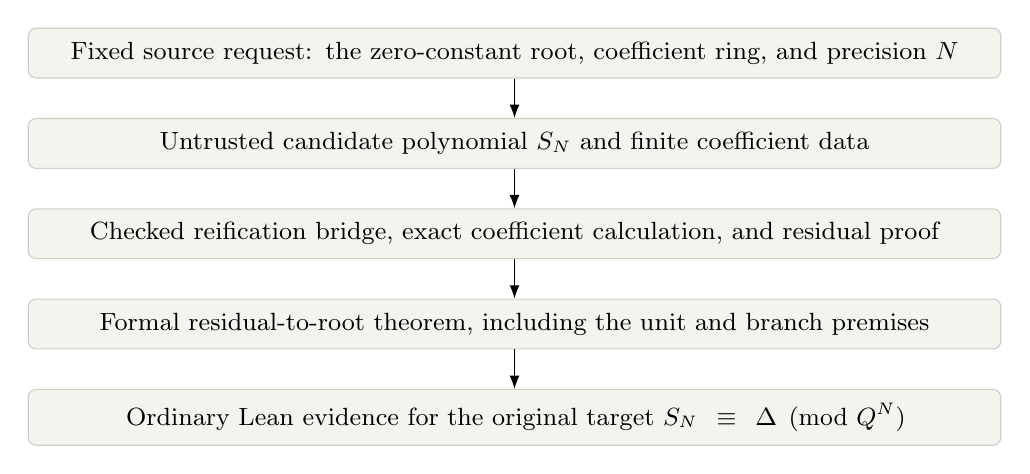
\begin{tikzpicture}[node distance=5mm, every node/.style={font=\small,align=center}, box/.style={draw=rulegray,fill=paperpanel,rounded corners=1mm,text width=12cm,inner sep=5pt}, >=Latex]
\node[box] (source) {Fixed source request: the zero-constant root, coefficient ring, and precision $N$};
\node[box,below=of source] (candidate) {Untrusted candidate polynomial $S_N$ and finite coefficient data};
\node[box,below=of candidate] (check) {Checked reification bridge, exact coefficient calculation, and residual proof};
\node[box,below=of check] (bridge) {Formal residual-to-root theorem, including the unit and branch premises};
\node[box,below=of bridge] (target) {Ordinary Lean evidence for the original target $S_N\equiv\Delta\pmod{Q^N}$};
\draw[->] (source)--(candidate);\draw[->] (candidate)--(check);\draw[->] (check)--(bridge);\draw[->] (bridge)--(target);
\end{tikzpicture}
\end{center}
A checker theorem about an encoded polynomial is not enough without the bridge between that encoding and the original source expression. Atom identities, variable order, coefficient ring, and arity are checked before combining coefficient arrays. Matching display names or relying on a digest as a proof of equality is insufficient.

Existing proof-producing algebra tactics are legitimate providers for the calculation. A new sparse-polynomial checker is not a prerequisite for every \Alder{} feature. If a new checker is introduced, its denotation and soundness theorems must be proved, and its execution path must fit the project's axiom policy. A native computation is not accepted merely because the abstract algorithm has a correctness theorem; the claimed result of that particular execution must be justified too.

\subsection{Analytic information is a separate upgrade, not a badge on the jet}
For this particular root, an analytic upgrade is available by a separate argument. Let $a_n$ be the coefficients in \eqref{eq:germclosed}. For $n\ge1$,
\[
 \left|\frac{a_{n+1}}{a_n}\right|
 =\frac{16}{9}\frac{4n-2}{n+1}\longrightarrow\frac{64}{9}.
\]
Thus the power series has radius of convergence $9/64$. For $|q|<9/64$ and $N\ge1$, the same ratio bound gives
\begin{equation}\label{eq:germ-error}
 \left|\Delta(q)-\sum_{n=1}^{N-1}a_nq^n\right|
 \le \frac{|a_Nq^N|}{1-(64/9)|q|}.
\end{equation}
Indeed, each subsequent term has absolute size at most $(64|q|/9)$ times its predecessor; summing the geometric majorant proves the bound. Substitution is legitimate by convergence, so this analytic series satisfies the equation and selects the branch near zero.

The formal statement $S_N\equiv\Delta\pmod{Q^N}$ does not imply \eqref{eq:germ-error} without this additional convergence and tail argument. In a proposed \Alder{} interface, asking for a real error bound would generate those analytic obligations, not silently promote the formal residual certificate. This is an example of a useful stronger property type whose evidence is explicit even when its routine derivation is automated.

\section{Behavioral synthesis over realizable observation frames}\label{sec:frames}

\subsection{The limitation of comparing raw affine coefficients}
Suppose a candidate's output length is an affine function of observed input lengths. Equality of two coefficient vectors is a sufficient test for equality on all length vectors. It need not be necessary on the vectors the source type can actually realize.

For a single \code{List Empty}, only length $0$ is possible. The affine expressions $0$ and $n$ therefore describe the same output-length law on that domain. For the pair of observations $(\operatorname{length}(xs),\operatorname{length}(\operatorname{reverse}(xs)))$, only the diagonal $(n,n)$ is possible. The expressions $n_1$ and $n_2$ agree there despite different coefficients. A Cartesian product of marginal possibilities would forget exactly this correlation.

The round-three reports separated positive soundness, decision completeness, negative realization, and observation coverage. The following theorem gives a concrete interface that supplies all the needed directions for a useful equality fragment without requiring the full observation image to be enumerated \cite{r3a,r3b}.

\subsection{A realizable affine frame}
\begin{definition}[Affine observation frame]\label{def:frame}
Let $X$ be a source input type, $D:X\to\mathsf{Prop}$ an admissibility predicate, and $\obs:X\to\Z^d$ an observation map. A realizable affine frame consists of admissible inputs $x_0,\ldots,x_m$ such that every admissible $x$ satisfies
\begin{equation}\label{eq:frame-cover}
 \obs(x)=b+\sum_{j=1}^m k_jv_j
 \quad\text{for some }k_j\in\Z,
 \qquad b=\obs(x_0),\quad v_j=\obs(x_j)-b.
\end{equation}
The data includes proofs of $D(x_i)$ and of this coverage statement. It need not assert that every integer combination in \eqref{eq:frame-cover} is itself realizable.
\end{definition}
The last sentence matters. A finite interval of possible lengths can have the same affine frame as all natural lengths. A diagonal observation family can have a one-direction frame although its ambient space is two-dimensional. The coverage used for positive reasoning may be an overapproximation, provided that the actual test points have concrete admissible realizations.

\Needspace{7\baselineskip}
\begin{theorem}[Finite decision by realizable affine observations]\label{thm:frame}
Let $G$ be an abelian group, and let $L,R:\Z^d\to G$ be affine maps: a constant plus an additive homomorphism. If $x_0,\ldots,x_m$ is a realizable affine frame, then
\[
 \forall x,\ D(x)\to L(\obs(x))=R(\obs(x))
 \quad\Longleftrightarrow\quad
 \forall i\in\{0,\ldots,m\},\ L(\obs(x_i))=R(\obs(x_i)).
\]
Any failing frame point is a concrete counterexample to the universal equality. If equality in $G$ is decidable, the finite comparison is a decision procedure; without that additional assumption, the result is a finite logical reduction rather than an executable decision procedure.
\end{theorem}
\begin{proof}
The forward implication follows by specialization to each admissible $x_i$. For the reverse implication put $H=L-R$, so $H(z)=c+\ell(z)$ with $\ell$ additive. Equality at $x_0$ gives $H(b)=0$. Equality at $x_j$ gives
\[
 0=H(b+v_j)=H(b)+\ell(v_j),
\]
so $\ell(v_j)=0$ for every direction. For any admissible $x$, use \eqref{eq:frame-cover} and additivity, including integer multiples, to obtain
\[
 H(\obs(x))=H(b)+\sum_{j=1}^m k_j\ell(v_j)=0.
\]
A failing test is already attached to an admissible $x_i$; specialization would contradict the claimed universal law. No surjectivity onto $\Z^d$ is required.
\end{proof}

\subsection{Source semantics must commute with the observation model}
Theorem~\ref{thm:frame} concerns affine maps. A candidate program is connected to it by a separate denotation theorem. For instance, for an exact candidate $c$ and source specification $s$ one needs
\begin{align*}
 \forall x,\ D(x)&\to \operatorname{length}(c(x))=L_c(\obs(x)),\\
 \forall x,\ D(x)&\to \operatorname{length}(s(x))=L_s(\obs(x)),
\end{align*}
with lengths embedded into $\Z$ when necessary. Only then does the finite frame comparison prove the source-level equality of lengths. It still says nothing about element order or permutation unless those have their own sound models and bridges.

An arbitrary black-box implementation that agrees on the frame can behave differently elsewhere. The affine model is justified by a source grammar or a theorem about that exact implementation. Finite tests alone do not supply it.

\subsection{The list grammar and its normalization theorem}
Consider a grammar with list variables, the empty list, cons by a fixed element, append, reverse, and map by a fixed total element function. Let $n_i$ be the input lengths. Associate an affine expression with each syntax node:
\begin{align*}
 \lambda([])&=0,&\lambda(x_i)&=n_i,\\
 \lambda(a::e)&=1+\lambda(e),&
 \lambda(e_1\mathbin{+\!+}e_2)&=\lambda(e_1)+\lambda(e_2),\\
 \lambda(\operatorname{reverse}(e))&=\lambda(e),&
 \lambda(\operatorname{map}(f,e))&=\lambda(e).
\end{align*}
Combining constants and coefficients computes an affine normal form.

\Needspace{7\baselineskip}
\begin{proposition}[Length-model soundness]\label{prop:lengthmodel}
For every well-typed expression $e$ in this grammar and every environment of lists,
\[
 \operatorname{length}(\operatorname{eval}(e,\text{env}))
 =\lambda(e)(\operatorname{length}(\text{env}_1),\ldots,
              \operatorname{length}(\text{env}_d)).
\]
\end{proposition}
\begin{proof}
Induct on the syntax of $e$. Empty lists and variables are immediate. Cons adds one to length; append adds the two lengths; reverse and map preserve length. Substitution of the induction hypotheses gives the stated affine equations. Coefficient collection preserves evaluation by associativity and distributivity of integer addition and multiplication.
\end{proof}
The grammar must itself be type-correct. A cons node over \code{Empty} requires an actual element of \code{Empty}; it cannot appear in a closed admissible program merely because an untyped length model permits ``add one.'' The Python interpreter uses lists of natural numbers and does not pretend to enforce Lean's element-type constraints for arbitrary external programs.

\subsection{Three frames, three different correct answers}
For $d$ independent \code{List Nat} inputs, take the all-empty environment and the $d$ environments with a singleton zero list in one coordinate. Their observations are $0,e_1,\ldots,e_d$. They cover all natural length vectors by nonnegative integer combinations and hence by \eqref{eq:frame-cover}. Equality of affine laws is equivalent to equality on these $d+1$ realizable probes.

For independent \code{List Empty} inputs, take only the all-empty environment. The direction family is empty. Every actual observation is zero, and only equality of constant terms matters. Comparing all raw coefficients would reject some true laws.

For the correlated observations of a list and its reverse, use the empty list and a singleton zero list. The frame observations are $(0,0)$ and $(1,1)$. An affine difference $c+a n_1+b n_2$ vanishes on all admissible inputs exactly when $c=0$ and $a+b=0$, not necessarily when $a=b=0$. A model-relative witness such as $(1,0)$ is not realizable and must not refute the source claim.

When $D$ has no admissible input, the universal claim is vacuous. No realizable base point $x_0$ exists. A separate proof of emptiness handles that case. An empty Python list of test points does not by itself certify that the source domain is empty.

\subsection{Why the coefficient domain matters}
The theorem uses integer affine combinations and an abelian group codomain. A rational linear-span test is a different theorem. Clearing denominators and then canceling an integer multiple can fail in a group with torsion. For example, $2g=0$ need not imply $g=0$.

Similarly, equality is essential to the affine-span argument. Agreement of inequalities at a collection of points does not extend to arbitrary signed affine combinations. Bounds can instead use a convex-hull coverage theorem with nonnegative weights, or a separately proved monotonicity argument. \Alder{} records the exact transport contract rather than treating every numeric observation as the same kind of evidence.

\subsection{How this fits Leant without replacing its existing design}
The Length source contract already carries exact spine identities, argument roles, provider transfers, and a joint pair-contract form \cite{lengthcontracts}. An \Alder{} adapter can augment that interface with:
\begin{enumerate}
\item A theorem linking the exact candidate's source semantics to the selected abstract transfer, including joint outputs.
\item A proof-backed frame or another explicitly stated coverage/realization interface for the admissible input domain.
\item A retained derivation connecting the successful finite check to the original frozen behavioral target.
\end{enumerate}
These are additional authorities, not inferred meanings of existing metadata. Ranking can continue to use inexpensive untrusted models. Acceptance requires the bridge. A negative outcome can be labeled \kw{model-relative counterexample} until the witness is realized at the source type; it becomes a \kw{checked candidate refutation} only after the exact negated source claim is proved.

The finite-frame theorem offers a sharper integration target than ``use SMT to understand behavior.'' It identifies a grammar, a domain theorem, a finite computation, and a precise source-level result. It also supplies a meaningful regression suite: independent, empty, and correlated input domains must yield different notions of equality.

\section{Relations, scopes, and mathematical proof moves}\label{sec:relations}

\subsection{Transport belongs to the consumer}
An evidence entry is not just ``$f$ equals $g$.'' It contains the actual proposition: equality of functions, equality on a set, eventual equality at a filter, almost-everywhere equality for a measure, or agreement below a power-series order. A registration states how a specified consumer respects that relation.

For example, neighborhood equality permits derivative transport at the neighborhood's point. Almost-everywhere equality permits the corresponding integral-congruence theorem for the fixed measure. A change of measure requires its own transport theorem. A coefficient truncation supports calculations in the relevant quotient ring. None of these relations is globally substituted for equality of all observations.

The exact premises come from the actual theorem signature. Some totalized operations admit congruence without existence or integrability assumptions that a more informative analytic result would require. \Alder{} should not impose generic guards that the selected theorem does not need; conversely, it must not omit the guards of a theorem asserting an actual derivative or a convergent sum.

\subsection{A useful nontrivial upgrade from almost everywhere}
There are legitimate routes from almost-everywhere to pointwise equality. A paper-level registration example is the following.

\Needspace{7\baselineskip}
\begin{proposition}[Continuity and full support]\label{prop:ae}
Let $X$ be a topological space equipped with a measure $\mu$ such that every nonempty open set has positive measure. If $f,g:X\to\R$ are continuous and $f=g$ almost everywhere with respect to $\mu$, then $f=g$ everywhere.
\end{proposition}
\begin{proof}
If $f(x_0)\ne g(x_0)$, continuity of $f-g$ implies that the set on which $f-g$ is nonzero is an open neighborhood of $x_0$. It therefore has positive measure. Almost-everywhere equality says exactly that this disagreement set has measure zero, a contradiction.
\end{proof}
The full-support premise is necessary for this route: a measure concentrated at one point need not distinguish continuous functions away from that point. A registered upgrade using Proposition~\ref{prop:ae} would permit subsequent point evaluation, but only after producing the additional evidence. This demonstrates why the property interface should be extensible by theorems, not hard-coded as a list of permanently incomparable badges.

\subsection{``Without loss of generality'' has a typed interface}
Many human proofs are shortened by symmetry. The abbreviation is justified when the language records both a normalization route and invariance of the target.

Let a group $G$ act on $X$, let $P:X\to\mathsf{Prop}$ be the target, and let $N$ be a normal-form predicate. Suppose
\[
 \forall x,\ \exists g:G,\ N(g\cdot x),\qquad
 \forall g\,x,\ P(g\cdot x)\leftrightarrow P(x).
\]
Then proving $\forall x,\ N(x)\to P(x)$ suffices to prove $\forall x,\ P(x)$. Choose the normalization witness for the fixed $x$, apply the normal-form theorem, and transport back by invariance. The witness remains scoped to this proof. No executable choice of normalizer follows merely from its proposition-valued existence.

A proposed command \code{wlog N by symmetry action} elaborates through precisely such a theorem. It does not guess that an expression looks symmetric. For a two-variable symmetric statement in a linear order, the chosen normal form might be $a\le b$, with the swap action and an explicit proof that swapping preserves the claim.

\subsection{Precision is an index, not a descriptive adjective}
Let $S\equiv_N T$ mean agreement below order $N$. Differentiation can use
\[
 S\equiv_{N+1}T\quad\Longrightarrow\quad S'\equiv_N T'.
\]
It generally cannot preserve $N$: $Q^N$ and $0$ agree below $N$, whereas their derivatives can differ at degree $N-1$. A request for an output jet of order $N$ can therefore propagate a demand for an input jet of order $N+1$. The requested output precision remains fixed; obtaining more input data is a delegated computation, not a change of statement.

This is an example of a requirement transformer already identified in earlier proposals. \Alder{} does not claim the idea as new. Its residual discipline supplies a uniform place to display the increased precision demand and a fixed boundary at which a certified producer may discharge it.

\section{Definition packages and universal properties}\label{sec:packages}

\subsection{A definition should export an evidence interface}
A mathematical definition package contains a carrier-level construction, its input structures, and separately named theorems about its result. It may also contain algorithms with proved correspondence to that construction. An author can request the part of the interface needed by the next proof step.

For a finite tensor-family construction, the data and guarantees should be separated conceptually:
\Needspace{128pt}
\begin{lstlisting}
construct W representing (T |-> forall i, AlgHom A (H i) T)
  using finite_tensor_family

request FiniteModule A W
request FreeModule A W
request Natural representing_equivalence
\end{lstlisting}
The representability request fixes the functor and the category of algebras. Finiteness and freeness are separate properties of the same constructed object. The naturality assertion concerns the entire family of equivalences and its behavior on algebra maps.

The inspected Lean source includes finite and free hypotheses for every factor when it requests those module properties \cite{tensor}. For a singleton family, the representing object is isomorphic to the sole factor. Taking $A=\Q$ and $H=\Q[X]$ shows that finite indexing alone cannot guarantee a finite-dimensional representing algebra. The property layer should surface the missing factor premises; it must not use a smaller index set as a proxy for a module bound.

\subsection{Bundling is a boundary decision}
Unbundled objects with local property proofs are often convenient while developing a proof. Bundled morphisms, subobjects, equivalences, and structures are often convenient at interfaces. \Alder{} should bridge these representations using explicit constructors and projection theorems.

For instance, a function together with a proved homomorphism law can be packaged as a homomorphism. A family together with a proved naturality law can be packaged as a natural transformation. In each case the construction must preserve the exact underlying function or family. It is not acceptable to synthesize a different morphism that merely satisfies a similar law and then pretend the original object has been refined.

Different constructions satisfying a universal property can be related by a canonical isomorphism \emph{after proving the relevant uniqueness theorem}. That is not definitional identity of their carriers. Dependent expressions on those carriers still require the isomorphism-specific transport appropriate to their consumer.

\subsection{Property learning is monotone; witness selection need not be}
Adding a new proof of $P(t)$ enriches the local evidence about the same $t$. Selecting a normalized representative, choosing a root, extending a partial function, or replacing a presentation by an isomorphic one introduces data. These operations may change subsequent computations and dependent types.

The source distinguishes \kw{know} from \kw{construct} for exactly this reason. A merge can usually combine new independent property proofs. Competing choices of a witness or structure can conflict, even when both choices are mathematically valid. A proof of uniqueness may later identify them propositionally, but a merge tool should not invent that proof or infer definitional equality from it.

\section{Implementation architecture and incremental correctness}\label{sec:implementation}

\subsection{An explicit pipeline}
The proposed Lean integration has six stages. First, parse the mathematical moves and elaborate their meaning-bearing terms. Second, record the fixed target, structure arguments, context, and allowed witness holes. Third, instantiate validated theorem registrations into a bounded graph. Fourth, solve proof obligations using the finite engine and selected external proof services. Fifth, reconstruct and check a Lean term for the exact target. Sixth, attach a source-linked receipt to the completed assertion or display its remaining conditional routes.

The output of one stage is typed input to the next. A solver cannot enlarge its authority by returning a different result kind. A candidate producer returns proposed data and evidence, not a declaration that it has changed the theorem. The final checker checks the exact elaborated target, not a string similarity score or a more convenient reformulation chosen by the producer.

\subsection{Evidence-index entry and identity}
A production evidence entry needs at least the following logical content:
\[
 (\Gamma\text{-snapshot},\ \text{proposition},\ \text{proof},\
   \text{source support},\ \text{structure footprint},\ \text{origin}).
\]
The proposition is an elaborated Lean expression, not a printed property name. Its arguments include all relevant types, universes, operations, topologies, measures, and dependent indices. The proof must be checked in the current context or imported through a verified context embedding.

Hashes are useful for lookup and invalidation. They are not proofs that two terms, contexts, or structures are equal. Exact expression comparison and kernel-checked transport remain the authority. Proof irrelevance can identify proofs of one proposition; it cannot identify two multiplication operations on the same carrier.

\subsection{A conservative answer to incremental elaboration}
The first implementation should rebuild the local evidence index for each elaborated declaration and discard it when the declaration is invalidated. It can retain global theorem registrations as an environment extension, but local facts must not survive by recycled local-variable identifiers.

A more aggressive cache may abstract a proof over its dependency telescope, retain that closed representation with environment dependencies, and instantiate it into a new context only after checking the substitution and resulting type. This is a typed context embedding problem. Generative epochs, as used in Leant's post-verification boundary, are good protection against accidental cross-batch association, but they do not by themselves prove that a dependent Lean context has been transported correctly \cite{postverification}.

The receipt is bound to a particular target, source edit, environment, and proof. After a dependency or toolchain change, rechecking issues a new receipt. A persistent green badge is not evidence that an old native result or stale local proof is valid in the new environment.

\subsection{What happens when simplification rewrites an anchor}
There are three cases. If the old and new elaborated expressions are definitionally equal in the current context, the proof can be reused through ordinary type checking. If simplification supplies a propositional equality or iff, create a transport edge and keep the old entry rather than silently changing its anchor. If neither applies, the new expression requires new evidence.

For dependent indices, the transport itself can change the type of the object. An element of $\operatorname{Fin}(n+1)$ is not an element of $\operatorname{Fin}(m)$ merely because a printer displays similar arithmetic. A proof of $n+1=m$ allows a dependent cast, and the consumer must see the cast or a proved equivalent interface. Simplifier normal forms are not globally canonical object identities.

The initial implementation can be conservative: keep proof-carrying rewrite edges only within the current declaration and reindex after a major goal transformation. The cost can then be measured before designing a persistent congruence structure for every kind of property.

\subsection{Proof sharing and the cost of elaboration}
Repeatedly inlining the same transport or guard can create large proof trees even when the source is short. Store proof DAGs and emit shared local bindings. Export useful repeated derivations as helper theorems when appropriate. Record at least the number of nodes, retained support sets, rule instantiations, generated term size, and time spent in final checking.

This does not establish that sharing is always a net win. A large index can cost more than calling an existing tactic. An aggressively opaque helper can change simplification behavior. The ordinary-Lean baseline must receive the same helper theorems and services, so the measurement isolates the interface rather than rewarding \Alder{} for owning a better library.

\subsection{Structure contexts do not erase instance search problems}
A lexical structure context fixes the relevant dictionaries for a block and can make their choices inspectable. It may reduce repeated setup and accidental changes. It cannot be assumed to remove all generated instance-disabling preambles in the Fermat corpus: those preambles may reflect elaboration search interactions not solved by merely naming a dictionary.

The proposed experiment is to instrument one real file, preserve the selected structures explicitly, and compare the remaining setup and search behavior. This article does not report such a run. It also does not register every learned proposition as a global typeclass instance, which would risk recreating the very search pollution the layer is meant to avoid.

\section{Should Lean's kernel type system change?}\label{sec:kernel}

\subsection{The first extension can be real without being trusted}
A source-level \code{requires} binder is more than a comment: the typechecker generates and discharges an obligation at each application, and the resulting declaration has an explicit proof argument in Lean. A behavioral arrow is more than an annotation: crossing the interface requires a function together with a theorem about that exact function. A residual type is more than an error message: it denotes a conditional term whose telescope can be checked.

These are meaningful type-system extensions at the authoring level. Their translation can use ordinary Lean $\Pi$-types, propositions, subtypes, structures, and equality elimination. This is the recommended implementation, because the remaining risks are predominantly in elaboration, dependency tracking, and usability, not in logical expressiveness.

\subsection{An explicit-evidence primitive refinement former}
A candidate kernel experiment would add a primitive type $\AlderRef(A,P)$ with rules equivalent to
\[
 \frac{a:A\quad h:P(a)}{\langle a,h\rangle:\AlderRef(A,P)},
 \qquad \frac{r:\AlderRef(A,P)}{\operatorname{val}(r):A},
 \qquad \operatorname{property}(r):P(\operatorname{val}(r)).
\]
Its essential computation rules would reduce projections on constructors. Subsumption would still require evidence:
\[
 \mathsf{weaken}(r,k):\AlderRef(A,Q),\qquad
 k:\forall a,\ P(a)\to Q(a).
\]
The expected ordinary-Lean translation is a subtype. An explicit introduction without $h$ would merely move the missing proof somewhere else, or change the logic.

Crucially, $\AlderRef(A,P)$ must not be definitionally identified with $A$. With $P$ constantly false and $A$ inhabited, such an identification together with a property projection would manufacture a proof of false. Erasing the proof field from compiled runtime representation is not the same as identifying the types in the kernel.

\subsection{What could a primitive improve?}
A primitive might make certain elaboration annotations cheaper to retain, make a projection representation more uniform, or enable a carefully restricted normalization of coercion composition. Those are engineering hypotheses. Ordinary Lean already erases proposition proofs from executable code and identifies proofs of the same proposition through proof irrelevance \cite{leanref}. Many same-carrier refinement paths therefore have little or no computational distinction to remove.

A genuine cost case would have to exhibit repeated dependent transports or coercion-normalization work that optimized ordinary encodings cannot remove. It would then compare the primitive against those optimized encodings, including shared proofs and better theorem interfaces. Without that experiment, ``kernel refinement types will be faster'' is not an evidence-backed conclusion.

\subsection{Definitional functoriality is a separate, nontrivial experiment}
Some verbosity arises from maps and transports that compose propositionally but do not normalize to the same term. The research on definitional functoriality for dependent subtypes studies adding selected functor laws to definitional equality and justifying structural coercive subtyping; its mechanized result concerns a specifically designed dependent type theory with list functor laws, not a drop-in proof that arbitrary extensions of Lean are safe \cite{functoriality}.

For \Alder{}, a plausible research prototype would choose one container family and explicit coercion maps, formulate the desired computation rules, and prove that translation preserves typing and the new conversions. Merely observing that a law is propositionally provable in Lean is insufficient: using it as conversion under dependent types can require inserted transports. One must analyze coherence, substitution, reduction, and the behavior of the actual checker.

Lean4Lean provides relevant infrastructure and results for studying Lean's type theory and checker. The current cited paper reports correctness results for parts of the kernel; this is not a blanket completed verification of every future kernel change \cite{lean4lean}. A refinement or coercion experiment would need its own metatheoretic and implementation argument.

\subsection{Semantic subtyping is not the default conversion relation}
A judgment $\AlderRef(A,P)\le\AlderRef(A,Q)$ may be justified by a theorem $\forall x,\ P(x)\to Q(x)$. The elaborator can search for that theorem and insert a coercion. Installing unrestricted theorem search inside definitional conversion is a different design: ordinary type checking would now inherit the behavior of an open-ended proof search procedure.

A bounded search timeout means unknown, not false. Keeping that search outside conversion allows the kernel to check the explicit successful result using its existing rules. The proposal does not rely on a simplistic claim about all aspects of Lean conversion being decidable; its point is to avoid adding arbitrary mathematical entailment as an implicit conversion obligation.

\subsection{Computational witnesses must not disappear into propositions}
An \code{IsUnit a} proof is a proposition about $a$. An actual unit value also carries an inverse, which can be computational data. A classical mathematical construction may recover a witness noncomputably. An executable operation needs an available constructive witness or a verified algorithm that computes it.

Likewise, existence and uniqueness of a root do not automatically give an executable infinite-series representation. The recurrence in Proposition~\ref{prop:germcoeff} supplies a finite-coefficient algorithm for this example; that algorithm is additional content. \Alder{} keeps the distinction between a mathematical object with certified properties and a program with certified behavior.

\subsection{Recommended decision}
Implement property-implicit binders, behavioral interfaces, and residual inference above the existing kernel. Treat a primitive refinement former as a measured representation experiment, and definitional functoriality as a separate research project with explicit metatheory. Do not make the authoring-language prototype depend on either. This gives the user richer mathematical types immediately while preserving an ordinary Lean proof artifact as the final authority.

\section{The executed Alder-0 artifact}\label{sec:executed}

\subsection{The actual grammar}
The shipped frontend has the following line-oriented grammar. Identifiers are opaque proposition names, not Lean terms. Comments begin with \texttt{\#}.
\Needspace{170pt}
\begin{lstlisting}
atoms P Q R
rule step : P & Q -> R
assume P
repair Q
explain R
begin local
  assume Q
  show R
end
\end{lstlisting}
Atom and rule declarations precede proof work. \code{assume} introduces an explicit hypothesis; \code{repair} sets the allowed missing-premise vocabulary; \code{explain} computes alternatives without extending the known facts; \code{show} requires the empty support. Lexical blocks restore the parent's facts and repair vocabulary when they end. They are scope tests, not an implementation of case elimination.

Every \code{show} is checked, including an assertion unused by the rest of the document. A module with a failed \code{show} produces no new output files through the command-line path. Conditional explanations generate explicitly conditional theorem text, never an unconditional proof of their targets.

\subsection{The independent derivation checker}
Proof nodes have three constructors: known assumption, permitted missing premise, and registered rule application. The checker verifies exact active assumption identities, target identity, rule identity, premise order, arity, and recursively computed residual support. It detects cycles and does not trust support annotations computed by the inference engine.

The checker is written separately from the saturation loop. This is useful defense against bookkeeping mistakes, not formal verification of the checker itself. A Python error shared by both implementations remains possible. The finite tests compare the inference result against a third, simple Boolean forward-closure oracle.

\subsection{Generated Lean and its explicit boundary}
A successful proof or residual is rendered as a theorem with opaque proposition parameters and explicit rule hypotheses. A typical output has this shape:
\Needspace{100pt}
\begin{lstlisting}
theorem sample (P Q R : Prop)
    (r : P -> Q -> R) (hP : P) (hQ : Q) : R := by
  have p0 : R := r hP hQ
  exact p0
\end{lstlisting}
The real generator shares proof DAG nodes through local \code{have} declarations and assigns internal identifiers rather than injecting source identifiers into Lean syntax. The files contain no \code{sorry} placeholders and do not declare the registry's mathematical laws as axioms. The laws are theorem parameters. Thus the generated terms express the verified \emph{propositional implication structure}; they do not establish that an arbitrary rule name denotes a true fact about integers, derivatives, or roots.

No Lean executable was available in the inspected environment. These generated files were not kernel-checked here. The package gives commands for that additional check, and the article never attributes fresh Lean acceptance to them. The richer \Alder{} examples elsewhere in the article are a proposed surface, not accepted input to this small parser.

\subsection{Executed results and their units}
The test run used Python 3.13.5 and the standard library. The complete result, including runtime and source hashes, is retained in \code{evidence/test_results.json}.
\begin{center}\small
\begin{tabularx}{\textwidth}{@{}Y r@{}}
\toprule Executed family & Count\\\midrule
Directed unary rule graphs on three atoms, excluding self-edges & 64\\
All known-seed and repair-vocabulary configurations for those graphs & 4,096\\
Independent support-subset closure probes for that family & 13,824\\
Returned derivations independently checked in that family & 11,904\\
Deterministically generated five-atom conjunctive rule graphs & 200\\
Support-subset oracle probes for the conjunctive family & 1,617\\
Returned derivations independently checked in that family & 934\\
Expected parser/checker/budget/cycle rejections & 16\\
Accepted authored proof or explanation requests in two examples & 4\\
Generated list-grammar expressions & 300\\
Concrete interpreter versus affine-model comparisons & 19,200\\
Affine-form pair/frame comparisons across three domain kinds & 46,875\\
Observation arity rejection & 1\\
Formal-root coefficients checked against the closed formula & 33\\
Perturbed root-jet residual checks & 48\\
Wrong-branch and nonunit arithmetic controls & 2\\
\bottomrule
\end{tabularx}
\end{center}
All these tests passed. The rows have different units and should not be summed into a fictitious count of formal theorems. ``Exhaustive'' applies only to the explicitly enumerated three-atom unary-graph family, not to all Horn theories. The list and affine arithmetic checks are finite executions, not kernel proofs of Propositions~\ref{prop:lengthmodel} or Theorem~\ref{thm:frame}.

The affine frame tests compare all pairs from 125 affine forms against independent, empty, and diagonal observation domains. The root tests confirm the coefficient formula through degree 32, check zero residual at that truncation, and alter coefficients to ensure the residual detects the change at the expected order. A second exact branch deliberately passes the residual test and fails the zero-constant branch condition. That is the desired outcome, not a broken checker.

\subsection{What has advanced beyond a paper policy}
There is now authored input with scope, a parser, an explicit finite inference computation, proof DAG construction, a separate validation pass, and generated conditional Lean source. The earlier reports' objection that a property engine was mostly a policy description is addressed for this narrow propositional part.

What has not advanced is equally specific: no mathematical theorem registry is linked to Lean, no actual Lean expression is reified by this frontend, no dependent context is cached across Lean edits, and no user study measures authoring benefit. The unit tests do not exercise imports changing typeclass choices, full \code{simp} transports, actual universes, or kernel trust-policy migration. Those remain integration tests, not silently counted among the passing Python cases.

\section{Evaluation that can distinguish a language from better automation}\label{sec:evaluation}

\subsection{The first production slice}
The first Lean implementation should expose one property-implicit binder and one method application around exact quotient transport. Use the satisfiable arithmetic contract of Section~\ref{sec:frey}, a small validated rule registry, and an obligation view. An ordinary Lean version must use the same extracted helper theorems. The next slice should connect the list grammar and a proved affine observation frame to Leant's exact candidate boundary.

Only after those two paths work from authored source to checked original-target evidence should the mathematical surface expand. The autonomous-derivative and formal-root examples in this article are already development material; they are not held-out transfer tasks. A genuinely held-out local-analysis task should be selected by an independent evaluator after the rule registry and interface have been fixed.

\subsection{Matched controls}
The comparison should distinguish the following layers rather than assign every improvement to syntax:
\begin{center}\small
\begin{tabularx}{\textwidth}{@{}P{.12\textwidth}Y@{}}
\toprule Arm & Available capabilities\\\midrule
$L_0$ & Current ordinary Lean with its existing automation.\\
$L_1$ & The same new mathematical packages and registered helper theorems as Alder, used through ordinary Lean.\\
$L_2$ & $L_1$ plus the same synthesis, arithmetic, certificate, and search services.\\
$L_3$ & $L_2$ plus property-implicit application and the typed residual interface.\\
$L_4$ & $L_3$ plus the richer mathematical proof-move surface.\\
$L_R$ & An appropriate ordinary-Lean arm with the same compact read-only renderer, but without the new input language.\\
\bottomrule
\end{tabularx}
\end{center}
This follows the controlled-comparison logic of the round-three syntheses \cite{r3a,r3b}. Current \code{fun_prop} already decomposes functions, uses registered function-property theorems, and discharges local hypotheses. Its documentation also identifies transition rules as a source of search growth and provides controls for their depth. It is therefore both a baseline and a source of implementation lessons, not a straw man \cite{funprop}.

\subsection{What to measure}
Record author interventions, time to a correct accepted proof, failure-diagnosis time, edit-repair work, and the reader's recovery of the exact mathematical statement. Record computational quantities separately: admitted rule instances, rule firings, antichain sizes, proof DAG nodes, term size, final checking time, and rebuild cost.

Line count can describe a source artifact but cannot establish usability. A one-line opaque invocation may be harder to understand and maintain than six explicit lines. Conversely, asking a reader to expand every automatically solved guard defeats the intended abstraction. The reading test should ask specifically about hidden-risk distinctions: domain, measure, branch, precision, admissible inputs, uniqueness, and completeness of a solution set.

\subsection{Paired mutations, with meaningful positive fixtures}
Each production acceptance test needs a satisfiable positive fixture, a single specified mutation, and an expected kind of failure. A representative matrix is:
\begin{center}\small
\begin{tabularx}{\textwidth}{@{}P{.28\textwidth}Y P{.18\textwidth}@{}}
\toprule Positive fixture & Mutation and required response & Status here\\\midrule
Open-region derivative identity & Retain only a point identity; local differentiation stays unresolved. & Paper/source example\\
Frey arithmetic at $(3,2,5)$ & Remove a divisibility premise; exact-quotient route exposes the guard. & Paper/source example\\
Zero-constant formal root & Use the other exact branch; residual success must not certify the requested branch. & Exact arithmetic control\\
Valid finite derivation & Change target, arity, rule, or active assumption; independent checker rejects. & Executed\\
Local block proof & Reuse its assumption after the block; publication fails. & Executed\\
Correct terminal assertion & Add an unrelated unproved assertion; module fails despite the earlier success. & Executed\\
Correlated length pair & Offer $(1,0)$ as a diagonal observation witness; no source refutation. & Paper theorem and arithmetic tests\\
Unchanged typed context & Recycle identifiers after rebuild or alter a dependent index; require recheck or transport. & Proposed integration test\\
Fixed structure instance & Change imports so another structure is selected; invalidate the sealed meaning or ask for a choice. & Proposed integration test\\
\bottomrule
\end{tabularx}
\end{center}
A shape-only Python model of the last two cases would not count as testing Lean's actual behavior. They must eventually be exercised in the real frontend.

\subsection{A legitimate stopping outcome}
If $L_3$ does not improve authoring and diagnosis over $L_2$, retain the library, synthesis bridge, and editor obligation view. If $L_4$ increases reader misunderstanding or maintenance cost relative to $L_3$ and $L_R$, drop the separate mathematical syntax. If a primitive refinement type does not beat an optimized ordinary encoding on a documented bottleneck, leave the kernel unchanged.

These are not reasons to avoid the experiment. They identify what would count as learning from it. A reusable proof-producing contract library and a correct residual explorer are useful artifacts even if the best eventual language remains ordinary Lean.

\section{Relationship to earlier type-theoretic work}\label{sec:related}
Refinement-based synthesis is established research. Synquid uses polymorphic refinement types to guide synthesis and decompose specifications. Its tractable checking and synthesis fragment does not make arbitrary Lean propositions decidable. \Alder{} borrows the specification-directed viewpoint but makes the boundary of its automatic fragment and the retained Lean evidence explicit \cite{synquid}.

Explicit refinement systems distinguish logical specifications from computational contents, while work on logical-framework refinements relates refinement interpretation to proof irrelevance. These are relevant precedents for separating a carrier from its proved properties. They do not remove the need for source interpretation, witness scope, or a concrete translation into Lean \cite{explicitref,lovas}.

Dijkstra monads connect effectful computation to predicate transformers and verification conditions. \Alder's residual mechanism is related in its backward flow of demands, but an unfinished mathematical justification is not itself an effectful program. The integration should reuse established program-verification semantics rather than invent an informal analogy in place of one \cite{dijkstra,mvcgen}.

Definitional functoriality and Lean4Lean are relevant to the optional kernel research described in Section~\ref{sec:kernel}. Neither is required for the initial frontend. Existing Lean function-property automation is the immediate engineering comparison \cite{functoriality,lean4lean,funprop}.

Finally, the nine round-three proposals supply most of the architectural baseline: same-object views, scope-closed support, separate structure selection, relational contracts, precision demands, and checked computation. \Alder's distinct emphasis is the executable residual calculus, the realizable affine-frame interface, and a source-facing conditional-proof discipline. The article builds on the syntheses' corrections instead of treating their convergence as independent experimental evidence \cite{r3a,r3b}.

\section{Conclusion}
A concise proof language should not try to make mathematics rigorous by guessing more aggressively about what the author meant. It should preserve that meaning and make the omitted justification a tractable, inspectable interface.

\Alder{} proposes three main mechanisms. First, fixed mathematical objects acquire proved property views, while proof-producing steps carry explicit residual telescopes until their obligations are discharged. Second, a finite grounded fragment computes alternative sufficient premise sets with proof DAGs, and reports its boundary rather than confusing incomplete search with falsity. Third, behavioral synthesis can use finite realizable observation frames when a source denotation theorem and an affine coverage theorem justify them.

The exact-quotient, local-differentiation, and algebraic-root examples show why these mechanisms matter: the missing evidence is often routine, but its type distinguishes a correct proof from a subtly different claim. The executable companion tests the central finite inference and authoring path. The remaining task is a small Lean implementation and an honest comparison with equally equipped ordinary Lean, not another expansion of the feature catalogue.

\clearpage\appendix
\section{Answers to the two sets of fourth-round questions}\label{app:questions}
The labels A1--A10 follow \emph{From Properties to Proof Obligations}; B1--B10 follow \emph{Nine Refinements}. The entries summarize an answer or explicitly identify work not executed here.
\begingroup\small
\begin{longtable}{@{}P{.08\textwidth}P{.30\textwidth}P{.55\textwidth}@{}}
\toprule Id & Question & Alder's answer and evidence boundary\\\midrule\endfirsthead
\toprule Id & Question & Alder's answer and evidence boundary\\\midrule\endhead
\bottomrule\endfoot
A1 & First use-site interface? & One exact-quotient property-implicit binder and method application; compare with the same helper in Lean. Alder-0 parses only its abstract propositional support model, not the real binder.\\
A2 & Finite automatic fragment? & Finite typed arena, bounded first-order theorem instantiation, then Horn antichain closure. Completeness is relative to the materialized rules. Sections~\ref{sec:inference}--\ref{sec:grounding}.\\
A3 & What data may inference choose? & Only witness holes explicitly delegated under a fixed specification. Structures, representations, and statement-determining holes are fixed or exposed as ambiguity. Section~\ref{sec:types}.\\
A4 & Required methods? & Restrict helper context and allowed registry before inference. A finite derivation-policy automaton is a possible extension; not implemented. Section~\ref{sec:inference}.\\
A5 & First behavioral bridge? & The list-expression affine model with a realizable affine frame. Paper proofs and exact tests here; Lean normalization and source reification remain to be linked. Section~\ref{sec:frames}.\\
A6 & Negative Leant selection? & A concrete admissible counterexample plus source transfer, or an exact proved negation. Unrealisable and merely model-relative witnesses do not refute the candidate.\\
A7 & First nonalgebraic transfer? & A held-out local-analysis task selected after the interface is frozen. The derivative theorem inspected here is development material, not a held-out result.\\
A8 & Retained/rechecked evidence? & Exact target, proof, context, source correspondence, structures, provider theorem dependencies, and policy. Rebuild local indices first; typed context embeddings are a later optimization. Section~\ref{sec:implementation}.\\
A9 & Performance gate for larger checkers? & Instrument a real file and compare against existing tactics under a chosen trust policy. The fast Python experiment is not that result.\\
A10 & When end the separate language? & Keep only library/services/editor views if the property or narrative layer gives no advantage against matched controls. Section~\ref{sec:evaluation}.\\\midrule
B1 & Evidence-index cost on a real file? & Not measured here. The Python result reports finite-graph counts only; production metrics are specified in Section~\ref{sec:evaluation}.\\
B2 & Which rules actually fire? & The executable records aggregate rule-combination work. There is no measured Mathlib rule histogram or comparison with single-lemma lookup yet.\\
B3 & Does simplification break anchors? & Reuse by current definitional checking or retain an explicit equality/iff transport edge. Never rekey by printed strings. Section~\ref{sec:implementation}.\\
B4 & One reifier for many checkers? & Share a typed expression grammar and denotation interface where semantics genuinely agree. Each consumer still proves its own correctness and original-target bridge. The prototype has no Lean reifier.\\
B5 & Completeness of Leant abstractions? & Theorem~\ref{thm:frame} gives a concrete completeness criterion for affine equality on a covered realizable domain. It makes no blanket claim about every Length contract.\\
B6 & Almost-everywhere consumers? & Register exact integral congruence and other consumer theorems with fixed measure arguments. A pointwise upgrade can use continuity and full support. Section~\ref{sec:relations}.\\
B7 & Do lexical contexts shorten FLT preambles? & Unmeasured; dictionary selection is not assumed to solve all instance-search conflicts. Preserve the real file and test it.\\
B8 & Bounded rule generation? & Section~\ref{sec:grounding} gives a finite arena, explicit theorem-shape restriction, and the $t^k$ grounding bound. The prototype starts from already-ground rules.\\
B9 & What does a compact reader recover? & Specify a blinded recovery test for domain, measure, branch, precision, and quantifiers. No human reading study was run here.\\
B10 & Independent implementations? & The Horn contract and supplied oracle tests can be implemented independently. The separate Python checker is useful but is not a second production Lean frontend.\\
\end{longtable}
\endgroup

\section{Package contents and reproduction}\label{app:reproduce}
The archive contains the self-contained \code{Alder.tex}, its rendered PDF, the companion sources and authored examples, generated Lean and JSON traces, a source register, test results, build instructions, and file hashes. No font files or vendored dependencies are included.

From the package root, run:
\Needspace{114pt}
\begin{lstlisting}
python companion/test_alder.py
python companion/alder_core.py companion/examples/quotient.alder \
  --lean companion/generated/Quotient.lean \
  --events companion/generated/quotient.json
latexmk -pdf -interaction=nonstopmode -halt-on-error Alder.tex
\end{lstlisting}
Python 3.10 or newer is required by the companion. The retained run used 3.13.5. The test script writes a new result JSON including its actual runtime and current source hashes; runtime is not expected to be byte-reproducible across machines.

The generated Lean files can additionally be checked with an installed Lean toolchain:
\Needspace{72pt}
\begin{lstlisting}
lean companion/generated/Quotient.lean
lean companion/generated/Locality.lean
\end{lstlisting}
Those commands are reproduction instructions, not a record that they were executed here. The generated theorems use only basic propositions and implication structure. Real integration still needs instantiated mathematical theorem registrations and an exact source-target bridge.

\clearpage
\begin{thebibliography}{99}
\small\raggedright
\bibitem{r3a} Codex. \emph{From Properties to Proof Obligations: A Critical Synthesis of the Nine Round-3 Proposals}. Revised 6 September 2026. Brainstorm, revision \code{bf3333905995060870f8585e297ffc16f3fe7e86}. Main report and its convergence crosswalk. \url{https://github.com/VladimirReshetnikov/Brainstorm/blob/bf3333905995060870f8585e297ffc16f3fe7e86/docs/round-3/synthesis/unified-report.tex}.
\bibitem{r3b} Claude (Anthropic). \emph{Nine Refinements: Property-Aware Typing in a Mathematician's Proof Language over Lean}. Revised 6 September 2026. Same Brainstorm revision; main report and \code{appendix.tex}. \url{https://github.com/VladimirReshetnikov/Brainstorm/blob/bf3333905995060870f8585e297ffc16f3fe7e86/docs/round-3/unified_report/unified_report.tex}.
\bibitem{autonomous} V. Reshetnikov and contributors. \code{AutonomousIteratedDeriv.lean}. ProveIt, revision \code{24ce8bd743eaab64a91ce90725ea00f498d319d2}. \url{https://github.com/VladimirReshetnikov/ProveIt/blob/24ce8bd743eaab64a91ce90725ea00f498d319d2/Analysis/FabiusFunction/Lean/FabiusFunction/AutonomousIteratedDeriv.lean}.
\bibitem{germ} V. Reshetnikov and contributors. \code{AlgebraicInverseGerm.lean}. Same ProveIt revision. \url{https://github.com/VladimirReshetnikov/ProveIt/blob/24ce8bd743eaab64a91ce90725ea00f498d319d2/Analysis/FabiusFunction/Lean/FabiusFunction/AlgebraicInverseGerm.lean}.
\bibitem{frey} Anthropic and credited project contributors. \code{S_FreyPackage_freyCurveInt_map.lean}. \emph{Fermat's Last Theorem in Lean}, revision \code{aa2d8b34692b16c70f699536de0d8e75b9a3e9ef}. \url{https://github.com/anthropics/fermats-last-theorem/blob/aa2d8b34692b16c70f699536de0d8e75b9a3e9ef/P2M/Sol/S_FreyPackage_freyCurveInt_map.lean}.
\bibitem{tensor} Anthropic and credited project contributors. \code{S_Algebra_exists_algHom_equiv_pi.lean}. Same Fermat repository revision. \url{https://github.com/anthropics/fermats-last-theorem/blob/aa2d8b34692b16c70f699536de0d8e75b9a3e9ef/P2M/Sol/S_Algebra_exists_algHom_equiv_pi.lean}.
\bibitem{verification} V. Reshetnikov and contributors. \code{src/Leant/Synth/Verification.hs}. Leant, revision \code{3a40904be8a410d832d9ab6900b3d3e7b425eccb}. \url{https://github.com/VladimirReshetnikov/Leant/blob/3a40904be8a410d832d9ab6900b3d3e7b425eccb/src/Leant/Synth/Verification.hs}.
\bibitem{postverification} V. Reshetnikov and contributors. \code{src/Leant/Synth/PostVerification.hs}. Same Leant revision. \url{https://github.com/VladimirReshetnikov/Leant/blob/3a40904be8a410d832d9ab6900b3d3e7b425eccb/src/Leant/Synth/PostVerification.hs}.
\bibitem{lengthcontracts} V. Reshetnikov and contributors. \code{src/Leant/Synth/Length/Contract.hs}. Same Leant revision. \url{https://github.com/VladimirReshetnikov/Leant/blob/3a40904be8a410d832d9ab6900b3d3e7b425eccb/src/Leant/Synth/Length/Contract.hs}.
\bibitem{leanref} Lean team. \emph{The Lean Language Reference}, chapters on the type system, propositions, functions, and proof validation. Accessed 6 September 2026. \url{https://lean-lang.org/doc/reference/latest/The-Type-System/}.
\bibitem{funprop} The mathlib community. \emph{Mathlib.Tactic.FunProp}: function-property theorem registration, decomposition, and transition rules. Accessed 6 September 2026. \url{https://leanprover-community.github.io/mathlib4_docs/Mathlib/Tactic/FunProp.html}.
\bibitem{mvcgen} Lean team. \emph{The Lean Language Reference: The mvcgen Tactic}, overview of predicate-transformer semantics and verification conditions. Accessed 6 September 2026. \url{https://lean-lang.org/doc/reference/latest/The--mvcgen--tactic/Overview/}.
\bibitem{synquid} N. Polikarpova, I. Kuraj, and A. Solar-Lezama. Program Synthesis from Polymorphic Refinement Types. PLDI 2016. Preprint v3, 21 April 2016. \url{https://arxiv.org/abs/1510.08419v3}.
\bibitem{explicitref} J. E. Ghalayini and N. Krishnaswami. Explicit Refinement Types. 2023. \url{https://arxiv.org/abs/2311.13995}.
\bibitem{lovas} W. Lovas and F. Pfenning. Refinement Types for Logical Frameworks and Their Interpretation as Proof Irrelevance. \emph{Logical Methods in Computer Science} 6(4), 2010. \url{https://arxiv.org/abs/1009.1861}.
\bibitem{dijkstra} D. Ahman, C. Hri\c{t}cu, K. Maillard, G. Mart\'inez, G. Plotkin, J. Protzenko, A. Rastogi, and N. Swamy. Dijkstra Monads for Free. POPL 2017; extended preprint v3, 2019. \url{https://arxiv.org/abs/1608.06499v3}.
\bibitem{functoriality} T. Laurent, M. Lennon-Bertrand, and K. Maillard. Definitional Functoriality for Dependent (Sub)Types. ESOP 2024; extended version v2. \url{https://arxiv.org/abs/2310.14929v2}.
\bibitem{lean4lean} M. Carneiro. Lean4Lean: Verifying a Typechecker for Lean, in Lean. Preprint v3, 14 September 2025. \url{https://arxiv.org/abs/2403.14064v3}.
\end{thebibliography}
\end{document}
